% artigo.tex - compilar com pdfLaTeX (duas vezes), na pasta que contem figuras/
\documentclass[11pt,a4paper]{article}
\usepackage[utf8]{inputenc}
\usepackage[T1]{fontenc}
\usepackage{lmodern}
\usepackage[brazil]{babel}
\usepackage[top=2.5cm,bottom=2.5cm,left=2.5cm,right=2.5cm]{geometry}
\usepackage{amsmath,amssymb}
\usepackage{graphicx}
\usepackage{array,booktabs}
\usepackage{caption}
\usepackage{enumitem}
\usepackage{microtype}
\usepackage{textcomp}
\usepackage{url}
\usepackage[hidelinks]{hyperref}
\DeclareUnicodeCharacter{2264}{\ensuremath{\leq}}
\DeclareUnicodeCharacter{2265}{\ensuremath{\geq}}
\DeclareUnicodeCharacter{2208}{\ensuremath{\in}}
\DeclareUnicodeCharacter{222A}{\ensuremath{\cup}}
\DeclareUnicodeCharacter{2200}{\ensuremath{\forall}}
\DeclareUnicodeCharacter{2211}{\ensuremath{\sum}}
\DeclareUnicodeCharacter{03A3}{\ensuremath{\textstyle\sum}}
\DeclareUnicodeCharacter{03B2}{\ensuremath{\beta}}
\DeclareUnicodeCharacter{03BC}{\ensuremath{\mu}}
\DeclareUnicodeCharacter{03C0}{\ensuremath{\pi}}
\DeclareUnicodeCharacter{221A}{\ensuremath{\surd}}
\DeclareUnicodeCharacter{2308}{\ensuremath{\lceil}}
\DeclareUnicodeCharacter{2309}{\ensuremath{\rceil}}
\DeclareUnicodeCharacter{2212}{\ensuremath{-}}
\DeclareUnicodeCharacter{2026}{\ensuremath{\ldots}}
\newcolumntype{L}[1]{>{\raggedright\arraybackslash}p{#1}}
\newcolumntype{C}[1]{>{\centering\arraybackslash}p{#1}}
\captionsetup{font=small,labelfont=bf,labelsep=endash,skip=4pt}
\newcommand{\fonte}[1]{\par\vspace{2pt}{\footnotesize #1\par}}
\newcommand{\bibentrada}[1]{\par\noindent\hangindent=1.2em\hangafter=1 #1\par\vspace{4pt}}
\setlength{\emergencystretch}{3em}
\setlength{\tabcolsep}{4pt}
\renewcommand{\arraystretch}{1.12}
\renewcommand{\topfraction}{0.92}\renewcommand{\bottomfraction}{0.8}\renewcommand{\textfraction}{0.06}
\renewcommand{\floatpagefraction}{0.75}
\setcounter{topnumber}{3}\setcounter{bottomnumber}{2}\setcounter{totalnumber}{5}

\title{\textbf{Cobertura efetiva universal da Atenção Primária em Santa Luzia/MG:} localização de equipes e unidades básicas com cobertura, capacidade e acessibilidade espacial}
\author{Arthur Soares Guimarães \and Messias Inácio da Silva Carvalho \and Pedro Hassen Coura Vieira}
\date{Universidade Federal de Minas Gerais -- Escola de Engenharia\\ Pesquisa Operacional para Saúde -- Prof. João Flávio de Freitas Almeida\\ Belo Horizonte, 2026}

\begin{document}
\maketitle

\begin{abstract}
\noindent Este trabalho determina o plano de menor custo para que toda a população de Santa Luzia/MG (230.382 habitantes) tenha cobertura efetiva da Atenção Primária à Saúde (APS), entendida como unidade próxima, pelo trajeto na rede de ruas, e vaga em uma equipe de Saúde da Família (eSF), com até 3.500 pessoas por eSF. Um modelo de programação linear inteira mista decide quantas eSF criar, se em Unidades Básicas de Saúde (UBS) existentes, até o porte de cada uma, ou em UBS novas, e a qual unidade vai cada um dos 398 setores censitários, inteiro. O modelo base, lexicográfico (eSF, obras e distância), é comparado com um modelo integrado que minimiza o custo anual em reais do governo e da população. Hoje, 99,3\% da população tem unidade no raio, mas só 85,2\% tem também vaga. Para 100\% de cobertura (C1), são necessárias 16 eSF novas, 9 em UBS existentes e 7 em 7 UBS novas, com R\$~13,92 milhões em obras. Com meta de 99\%, bastam 10 eSF em UBS existentes, sem obra, e o último 1\%, rural e disperso, pode ser atendido por uma eSF volante de R\$~1,04 milhão por ano. Com os preços de referência, o modelo integrado chega às mesmas unidades do modelo base.

\medskip\noindent\textbf{Palavras-chave:} atenção primária à saúde; localização de unidades; programação linear inteira mista; cobertura efetiva; acessibilidade espacial.
\end{abstract}

{\renewcommand{\abstractname}{Abstract}\hyphenpenalty=10000 % texto em ingles: sem hifenizacao em portugues
\begin{abstract}
\noindent This study determines the least-cost plan for the whole population of Santa Luzia, Brazil (230,382 inhabitants) to have effective coverage of Primary Health Care, defined as a nearby facility, measured along the street network, and an available place in a Family Health team (up to 3,500 people per team). A mixed-integer linear programming model decides how many teams to create, whether in existing primary care facilities, up to their capacity, or in new ones, and to which facility each of the 398 census tracts is wholly assigned. The lexicographic base model (teams, construction, distance) is compared with an integrated model that minimizes the annual cost, in Brazilian reais, for the government and the population. Today, 99.3\% of the population has a facility within the maximum distance, but only 85.2\% also has an available place. Full coverage (C1) requires 16 new teams, 9 in existing facilities and 7 in 7 new facilities, with R\$~13.92 million in construction. With a 99\% target, 10 teams in existing facilities suffice, without construction, and the remaining 1\%, rural and scattered, can be served by a mobile team costing R\$~1.04 million per year. At reference prices, the integrated model selects the same facilities as the base model.

\medskip\noindent\textbf{Keywords:} primary health care; facility location; mixed-integer linear programming; effective coverage; spatial accessibility.
\end{abstract}}



\section{Introdução}

\subsection{Contexto}\label{sec:1.1}

A Atenção Primária à Saúde (APS) é a porta de entrada preferencial do Sistema Único de Saúde (SUS) e organiza o cuidado nas redes de atenção. No Brasil, ela se estrutura sobretudo pela Estratégia Saúde da Família (ESF): cada equipe de Saúde da Família (eSF) responde por uma população adscrita em um território definido (BRASIL, 2017). Planejar a APS é, portanto, decidir \textbf{quantas} equipes são necessárias, \textbf{onde} elas atuam e \textbf{quem} cada uma atende.

Santa Luzia, na Região Metropolitana de Belo Horizonte, tem população de referência de 230.382 habitantes em 233,76 km² e dois distritos, a Sede e São Benedito. A rede de APS conta com 28 Unidades Básicas de Saúde (UBS), 4 pontos de apoio rurais e 57 eSF. Em 2025, o município empenhou R\$~208,3 milhões em saúde, dos quais R\$~56,2 milhões na Atenção Básica, e aplicou 23,34\% da receita de impostos e transferências em ações e serviços públicos de saúde, acima do mínimo legal de 15\% (SANTA LUZIA, 2026).

\subsection{Problema}\label{sec:1.2}

O Relatório Anual de Gestão (RAG) de 2025 informa 97,3\% de ``população coberta pelas ESF'', razão entre os 224.101 usuários cadastrados e a população. O indicador mede \textbf{cadastro}, e não \textbf{capacidade}: as 57 equipes têm, em média, 3.932 cadastrados. O indicador de cobertura potencial do Ministério da Saúde, definido na Nota Técnica nº 2/2025-SAPS/MS, considera 3.500 pessoas por eSF e resulta em 86,6\% para o município (BRASIL, 2025a). Nenhum dos dois indicadores, porém, informa se as vagas estão \textbf{perto} de quem precisa delas.

Este trabalho adota a noção operacional de \textbf{cobertura efetiva} do acesso: um morador está coberto quando existe uma unidade de APS dentro de uma distância máxima, medida pelo trajeto na rede de ruas, \textbf{e} há vaga em uma equipe dessa unidade. A Seção~\ref{sec:2.2} mostra que essa medida corresponde ao componente de oferta e acesso potencial da cobertura efetiva de Shengelia et al. (2005), e não à medida completa, que inclui utilização e qualidade.

O porte de cada UBS, isto é, o número máximo de eSF que o prédio comporta, foi levantado por CNES. Somadas, as UBS existentes comportam 19 eSF além das atuais. O trabalho admite, assim, duas formas de criar vagas: acrescentar eSF nas UBS existentes, até o porte, sem obra, e abrir UBS novas, de porte I a V do Novo PAC Saúde.

\subsection{Objetivos}\label{sec:1.3}

O objetivo geral é determinar o plano de menor custo para elevar a cobertura efetiva da APS em Santa Luzia a 100\%. Os objetivos específicos são:
\begin{enumerate}[label=\alph*),leftmargin=*,itemsep=2pt]
\item diagnosticar a cobertura efetiva atual, com distâncias pela rede de ruas, e decompor a população descoberta em falta de vaga e falta de unidade próxima;
\item formular e resolver um modelo de programação linear inteira mista (o modelo base) que decida quantas eSF criar, se em UBS existentes ou novas, e a qual unidade cada setor censitário, inteiro, é vinculado;
\item comparar o modelo base, de objetivo lexicográfico, com um modelo integrado que minimiza o custo anual total em reais, separando o custo do governo e o da população;
\item avaliar cenários de distância máxima e de meta (incluindo uma eSF volante, com cronograma), a sensibilidade e a robustez do cenário principal;
\item medir, fora da otimização, a acessibilidade espacial (GUAGLIARDO, 2004), os encaminhamentos aos níveis secundário e terciário e o esforço orçamentário.
\end{enumerate}


\section{Referencial teórico}

\subsection{Acesso, necessidade, demanda e oferta}\label{sec:2.1}

Aday e Andersen (1974) propõem um quadro para estudar o acesso em que o sistema de prestação de serviços é descrito por seus \textbf{recursos}, isto é, o volume e a distribuição de pessoal e de estrutura, medidos por unidade de população e por unidade de área, e por sua \textbf{organização}, medida, entre outros, pelo tempo médio de deslocamento e de espera. Os indicadores de razão entre oferta e população e de distância usados neste trabalho pertencem a esse grupo de medidas do sistema.

Santana et al. (2023) distinguem necessidade, demanda e oferta e as combinam em sete situações. Duas delas interessam aqui: necessidade e demanda sem oferta suficiente, em que o acesso é restringido pela capacidade, e oferta sem necessidade nem demanda, que caracteriza capacidade ociosa.

\subsection{Cobertura efetiva}\label{sec:2.2}

Shengelia et al. (2005) definem cobertura efetiva como a probabilidade de um indivíduo obter o ganho de saúde de uma intervenção quando precisa dela. Para o indivíduo $i$ e a intervenção $j$:
\begin{equation}
\mathit{EC}_{ij} = Q_{ij} \cdot U_{ij} \mid N_{ij} = 1
\end{equation}

\noindent em que $Q_{ij}$ é a qualidade esperada, $U_{ij}$ é a utilização e $N_{ij}$ indica a necessidade (SHENGELIA et al., 2005).

A medida deste trabalho \textbf{não é} a de Shengelia et al. (2005). Ela considera necessidade $N_{i}$ = 1 para toda a população, porque a APS é universal, e verifica apenas se há unidade dentro da distância máxima e vaga em uma equipe. Corresponde, assim, ao componente de oferta e acesso potencial, que Guagliardo (2004) chama de disponibilidade e acessibilidade. Não inclui a utilização observada nem a qualidade, porque a base não contém produção de atendimentos por equipe nem ganho de saúde por prestador.

\subsection{Acessibilidade espacial}\label{sec:2.3}

Guagliardo (2004) distingue o acesso \textbf{potencial} do acesso \textbf{realizado}. Das cinco dimensões do acesso, duas são espaciais: a \textbf{disponibilidade}, o número de pontos de serviço entre os quais o morador pode escolher, e a \textbf{acessibilidade}, a impedância de viagem até esses pontos. A forma mais simples do modelo gravitacional é a de Hansen (1959):
\begin{equation}
A_i = \sum_{j \in J} \frac{S_j}{d_{ij}^{\,\beta}}
\end{equation}

\noindent em que $S_{j}$ é a capacidade de oferta do ponto $j$, $d_{ij}$ é a impedância entre a origem $i$ e o destino $j$, e $\beta $ é o coeficiente de decaimento com a distância. Joseph e Bantock (1982) acrescentaram a demanda potencial sobre cada ponto de serviço:
\begin{equation}
V_j = \sum_{k \in K} \frac{P_k}{d_{kj}^{\,\beta}}, \qquad A_i = \sum_{j \in J} \frac{S_j}{d_{ij}^{\,\beta}\, V_j}
\end{equation}

\noindent em que $P_{k}$ é a população do ponto de demanda $k$.

\subsection{Modelos de localização com cobertura e custo}\label{sec:2.4}

Do problema de cobertura de conjuntos (TOREGAS et al., 1971) e do problema de máxima cobertura (CHURCH; REVELLE, 1974) vem a ideia de que um ponto de demanda só é atendido dentro de um padrão de distância. Dos modelos de localização capacitada vem a exigência de que a unidade tenha capacidade para atender quem lhe é alocado, e da designação única, a de que cada ponto de demanda seja atendido por um só destino. A combinação aproxima-se da metodologia de Rocha et al. (2019), que delimita áreas de cobertura das equipes a partir de setores censitários, de proximidade e de um teto de pessoas por equipe.

Almeida et al. (2019) formulam a localização de centros de especialidades em Minas Gerais como um modelo inteiro misto que minimiza, numa única função em reais por ano, o custo de manutenção dos centros, a depreciação dos equipamentos e o \textbf{custo social de deslocamento} dos pacientes, com designação única de cada município a um centro e distâncias obtidas por um serviço de rotas. O custo de deslocamento por viagem soma a tarifa de transporte por quilômetro, em ida e volta, e o valor do tempo, dado pelo tempo de viagem multiplicado pela renda média por hora. Essa formulação é a base do modelo integrado deste trabalho (Seção~\ref{sec:3.6}).


\section{Metodologia}

\subsection{Sistema de saúde modelado e conceitos}\label{sec:3.1}

O sistema modelado é a \textbf{APS do SUS no município}, organizada pela Estratégia Saúde da Família. Os elementos e as definições adotadas são:
\begin{enumerate}[label=\alph*),leftmargin=*,itemsep=2pt]
\item \textbf{população adscrita}: cada setor censitário (unidade de demanda) é vinculado a uma unidade de APS; o setor é atendido inteiro por uma única unidade, e uma unidade atende vários setores;
\item \textbf{eSF}: equipe de Saúde da Família, com médico, enfermeiro, técnico ou auxiliar de enfermagem e agentes comunitários de saúde (BRASIL, 2017); a equipe de Atenção Primária (eAP), de 20 ou 30 horas, é admitida apenas na sensibilidade (BRASIL, 2019);
\item \textbf{UBS existente}: mantém as eSF atuais e pode receber eSF novas até o seu \textbf{porte}, o número máximo de eSF que o prédio comporta; \textbf{ponto de apoio rural}: local sem equipe própria, atendido pela equipe da UBS responsável;
\item \textbf{UBS nova}: projeto de porte I a V do Novo PAC Saúde (1 a 5 eSF), com custo de obra de referência (BRASIL, 2025b);
\item \textbf{cobertura efetiva} (sentido operacional): o morador tem uma unidade a até a distância máxima pela rede de ruas \textbf{e} vaga em uma eSF dessa unidade, com no máximo 3.500 pessoas por eSF.
\end{enumerate}

A Tabela \ref{tab:ms} resume os parâmetros do Ministério da Saúde usados no trabalho.

\begin{table}[!htb]
\centering
\small
\caption{Parâmetros do Ministério da Saúde}\label{tab:ms}
\begin{tabular}{@{}L{\dimexpr 0.3858\linewidth-2\tabcolsep\relax}L{\dimexpr 0.2646\linewidth-2\tabcolsep\relax}L{\dimexpr 0.3496\linewidth-2\tabcolsep\relax}@{}}
\toprule
\textbf{Parâmetro} & \textbf{Valor} & \textbf{Norma} \\
\midrule
Pessoas por eSF (cobertura potencial) & 3.500 & Nota Técnica nº 2/2025-SAPS/MS (BRASIL, 2025a) \\
Pessoas por eSF (cofinanciamento, mun. > 100 mil hab.) & 3.000 & Portaria GM/MS nº 3.493/2024 (BRASIL, 2024) \\
Capacidade da eAP 20h e 30h & 1.750 e 2.625 & NT nº 2/2025-SAPS/MS (50\% e 75\% da eSF) \\
Composição mínima da eSF & médico, enfermeiro, técnico/auxiliar, ACS & PNAB, Portaria nº 2.436/2017 (BRASIL, 2017) \\
Porte das UBS novas e custo de obra & I a V (1 a 5 eSF); R\$~1,988 a 5,214 mi & Novo PAC Saúde, Manual de Seleções 2025 (BRASIL, 2025b) \\
Repasse federal por eSF & R\$~24 mil por mês & e-Gestor APS (componentes fixo, vínculo e qualidade) \\
Consultas médicas por habitante por ano & 2 a 3 (63\% básicas) & Portaria GM/MS nº 1.101/2002 (BRASIL, 2002), revogada pela Portaria nº 1.631/2015 (BRASIL, 2015); usada como ordem de grandeza \\
\bottomrule
\end{tabular}
\fonte{Fonte: elaborada pelos autores.}
\end{table}

O \textbf{objetivo do modelo base} é, nesta ordem: usar o menor número de eSF novas; entre os planos com esse número, a menor obra; e, entre esses, a menor distância total percorrida pela população. O modelo integrado, de comparação, minimiza o custo anual total em reais.

\subsection{Área de estudo e dados}\label{sec:3.2}

A demanda é representada pelos 398 setores censitários do Censo 2022 (IBGE, 2023), cada um localizado no seu ponto central, com população ajustada proporcionalmente à estimativa do Ministério da Saúde para 2025 (230.382 habitantes). Os setores classificados pelo IBGE como ``área urbanizada de cidade ou vila'' são tratados como urbanos; os demais, como rurais. A Tabela \ref{tab:dados} resume as fontes.

\begin{table}[!htb]
\centering
\small
\caption{Dados e fontes}\label{tab:dados}
\begin{tabular}{@{}L{\dimexpr 0.4999\linewidth-2\tabcolsep\relax}L{\dimexpr 0.5001\linewidth-2\tabcolsep\relax}@{}}
\toprule
\textbf{Dado} & \textbf{Fonte} \\
\midrule
Setores censitários: população, área, situação e coordenadas & IBGE, Censo 2022 (IBGE, 2023) \\
População de referência (2025) & Ministério da Saúde, e-Gestor APS \\
UBS, eSF, unidades de média e alta complexidade e coordenadas & CNES (10/2026) e georreferenciamento do grupo \\
Porte de cada UBS (número máximo de eSF) & Planilha CNES-Porte, levantada pelo grupo por CNES \\
Rede de ruas & OpenStreetMap, rede a pé, obtida com o OSMnx (BOEING, 2017) \\
Usuários cadastrados por eSF & e-Gestor APS / SISAB \\
Custo de obra das UBS (porte I a V) & Novo PAC Saúde, Manual de Seleções 2025 (BRASIL, 2025b) \\
Despesa com saúde e com APS; repasse federal por eSF & RAG 2025 (SANTA LUZIA, 2026); e-Gestor APS \\
Renda média; salário mínimo & IBGE, Cadastro Central de Empresas 2021 (IBGE, 2023b); Decreto nº 12.342/2024 \\
Custo por quilômetro de transporte (eSF volante) & Central de Compras, Ministério da Economia (BRASIL, [2020]) \\
\bottomrule
\end{tabular}
\fonte{Fonte: elaborada pelos autores.}
\end{table}

O porte foi obtido para 27 das 28 UBS. Para UBS Cotegipe, sem dado, considera-se que não há espaço para novas eSF (porte igual ao número atual de equipes). A folga total é de 19 eSF, 11 na Sede e 8 em São Benedito, distribuída em 16 UBS (Figura \ref{fig:f23}).

\begin{figure}[!htb]
\centering
\caption{eSF atuais e porte de cada UBS existente}\label{fig:f23}
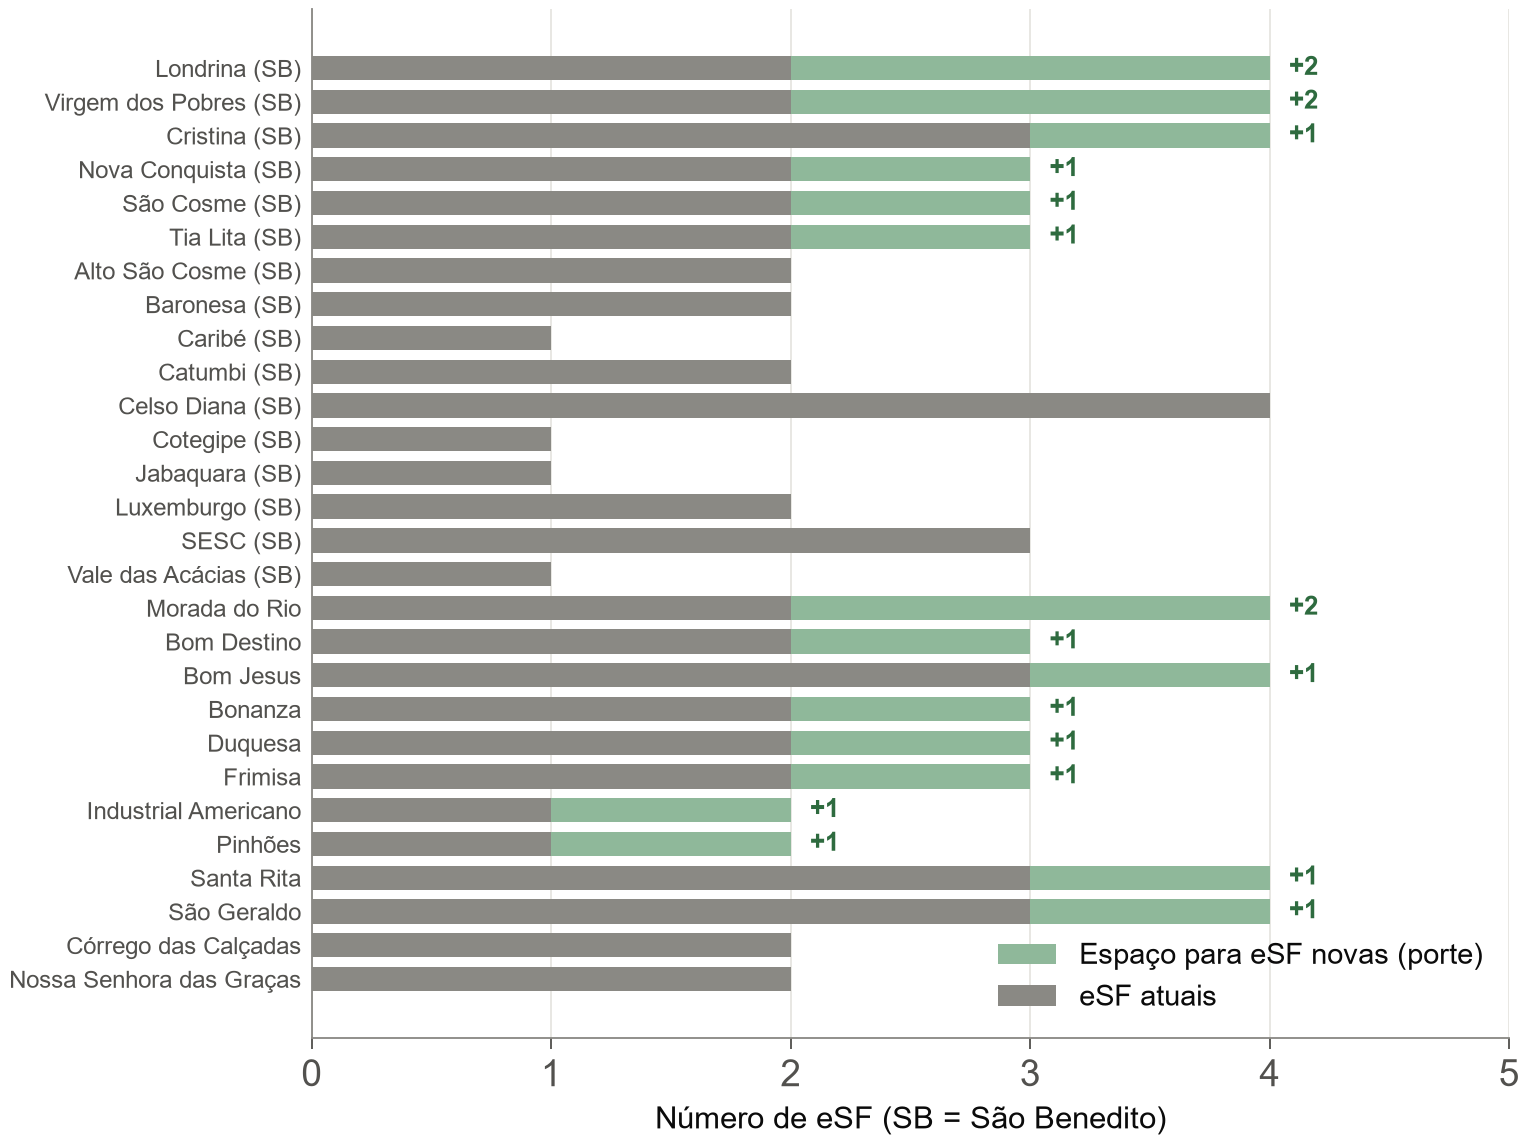
\includegraphics[width=0.79\linewidth]{figuras/f23_porte_ubs.png}
\fonte{Fonte: elaborada pelos autores com dados do CNES e da planilha CNES-Porte.}
\end{figure}

\subsection{Matriz de distâncias pela rede de ruas}\label{sec:3.3}

A matriz de distâncias é a entrada comum do modelo e dos índices de acessibilidade. Para cada origem $i$ (setor) e destino $j$ (UBS existente, ponto de apoio ou local candidato), $d_{ij}$ é a distância do \textbf{trajeto efetivo pela rede de ruas}. A rede de vias do município, com 1,5 km de margem, foi obtida do OpenStreetMap com o OSMnx (BOEING, 2017), na rede de pedestres, que inclui calçadas e vias de uso local e não impõe sentido de tráfego. Cada ponto é ligado ao nó mais próximo da maior componente conexa da rede; a distância é a soma da ligação do ponto à rede, do caminho mínimo na rede (algoritmo de Dijkstra) e da ligação da rede ao destino. A distância em linha reta (fórmula de Haversine) é mantida apenas para comparação e para a análise de sensibilidade. Pela rede, a distância é, em mediana, 1,32 vez a distância em linha reta (Figura \ref{fig:f22}).

\begin{figure}[!htb]
\centering
\caption{Distância pela rede de ruas e em linha reta, setor × unidade}\label{fig:f22}
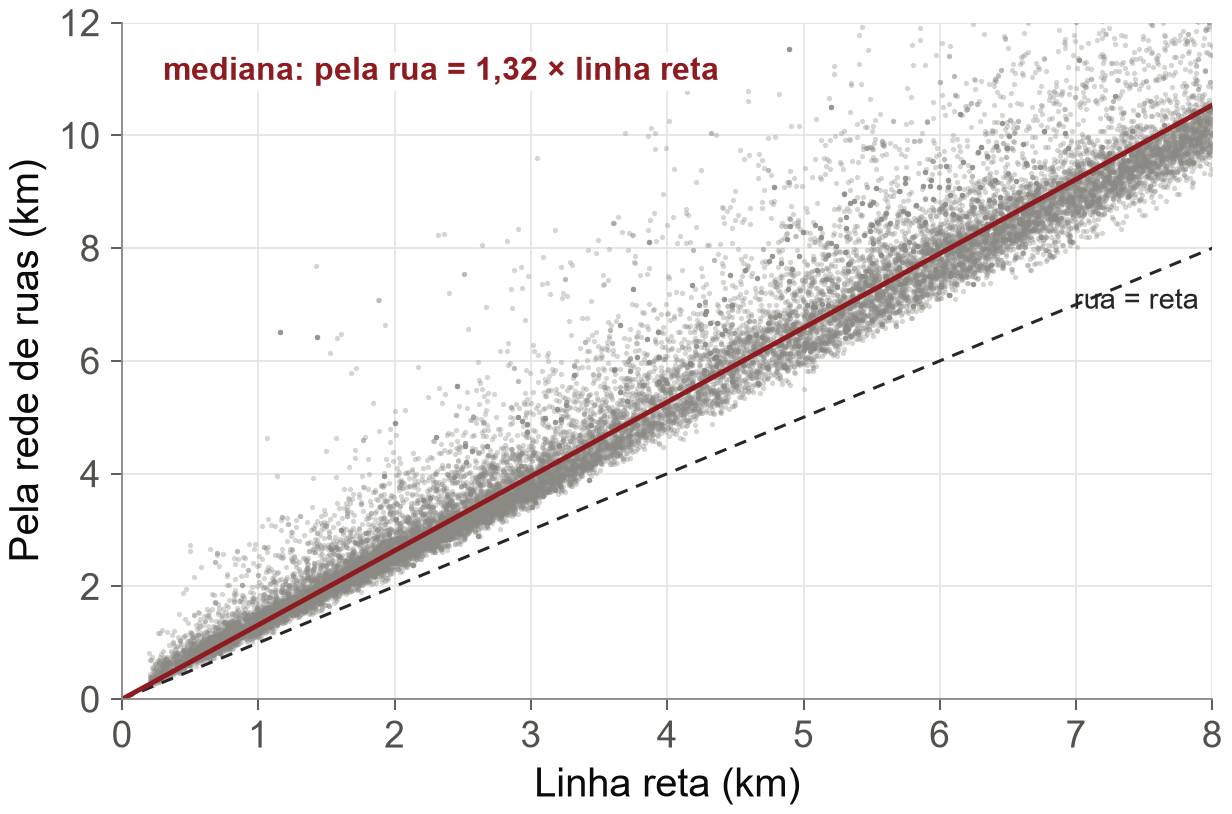
\includegraphics[width=0.79\linewidth]{figuras/f22_rede_reta.png}
\fonte{Fonte: elaborada pelos autores com dados do OpenStreetMap, do IBGE (2023) e do CNES.}
\end{figure}

Na notação da aula de acessibilidade, a matriz origem-destino $\mathit{Di}$ e a matriz demanda-destino $\mathit{Dk}$ coincidem, porque os pontos de demanda são os próprios setores. A matriz completa está nos arquivos matriz\_distancias.xlsx e matriz\_distancias\_rede.xlsx. A Figura \ref{fig:f04} mostra a distribuição da distância até a unidade mais próxima.

\begin{figure}[!htb]
\centering
\caption{Distribuição da população pela distância (pela rua) até a unidade de APS mais próxima}\label{fig:f04}
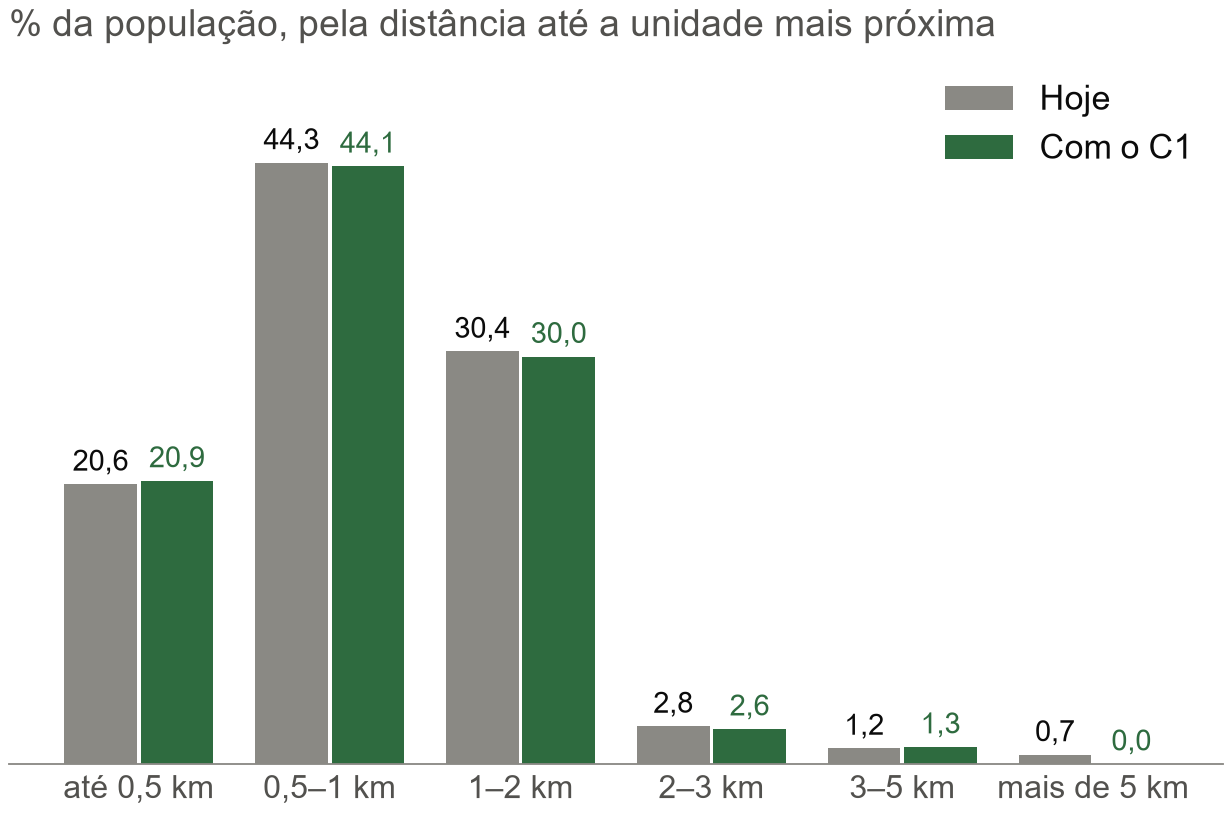
\includegraphics[width=0.89\linewidth]{figuras/f04_distancia_mais_proxima.png}
\fonte{Fonte: elaborada pelos autores com dados do IBGE (2023), do CNES e do OpenStreetMap.}
\end{figure}

\subsection{Parâmetros}\label{sec:3.4}

A Tabela \ref{tab:param} resume os parâmetros do modelo, com a fonte ou a justificativa de cada um; os valores alternativos são testados na análise de sensibilidade (Seção~\ref{sec:4.7}).

\begin{table}[!htb]
\centering
\small
\caption{Parâmetros do modelo}\label{tab:param}
\begin{tabular}{@{}L{\dimexpr 0.3417\linewidth-2\tabcolsep\relax}C{\dimexpr 0.2756\linewidth-2\tabcolsep\relax}L{\dimexpr 0.3826\linewidth-2\tabcolsep\relax}@{}}
\toprule
\textbf{Parâmetro} & \textbf{Valor} & \textbf{Fonte ou justificativa} \\
\midrule
Pessoas por eSF (parâmetro e limite) & 3.500 & NT nº 2/2025-SAPS/MS; 3.000 (Portaria nº 3.493/2024) na sensibilidade \\
Distância máxima, setor urbano & 3 km pela rua (C1, C3); 5 km (C2) & Premissa dos cenários \\
Distância máxima, setor rural & 5 km pela rua (C1, C3); 10 km (C2) & Premissa dos cenários \\
eSF novas nas UBS existentes & até o porte (+19 no total) & Planilha CNES-Porte; sem custo de obra \\
UBS nova & porte I a V (1 a 5 eSF) & Novo PAC Saúde: R\$~1,988 a 5,214 milhões \\
Locais candidatos & centro dos 398 setores & Critério alternativo (> 1 km de UBS) na sensibilidade \\
Pontos de apoio rurais & 4 & Só setores rurais; usam a vaga da UBS responsável (a mais próxima pela rua) \\
Atendimento do setor & inteiro, por uma única unidade & Setor dividido apenas na sensibilidade \\
Meta de cobertura efetiva & 100\% (C1, C2); ≥ 99\% (C3) & Definição dos cenários \\
\bottomrule
\end{tabular}
\fonte{Fonte: elaborada pelos autores.}
\end{table}

\subsection{Formulação do modelo base}\label{sec:3.5}

\textbf{Conjuntos.} $S$: setores; $U$: UBS existentes; $A$: pontos de apoio; $N$: locais candidatos; $T$: tipos de UBS nova; $J$ = $U$ ∪ $A$ ∪ $N$. O conjunto $L$ contém os pares ($i$, $j$) com $d_{ij}$ ≤ $D_{i}$, sendo $D_{i}$ a distância máxima do setor $i$; pontos de apoio só formam pares com setores rurais.

\textbf{Parâmetros.} $p_{i}$: população do setor $i$; $C$: pessoas por eSF; $e_{u}$: eSF atuais da UBS $u$; $g_{u}$: eSF que ainda cabem na UBS $u$ (porte − $e_{u}$); $\mu $($a$): UBS responsável pelo ponto de apoio $a$; $q_{t}$ e $c_{t}$: eSF e custo de obra do tipo $t$; $M$: meta de cobertura.

\textbf{Variáveis.} $x_{ij}$ ∈ \{0, 1\}: o setor $i$ é atendido, inteiro, na unidade $j$; $a_{u}$ ∈ \{0, 1, …, $g_{u}$\}: eSF novas na UBS existente $u$; $w_{kt}$ ∈ \{0, 1\}: abre-se no local $k$ uma UBS do tipo $t$.

\textbf{Objetivo lexicográfico.} Os três critérios são minimizados em sequência, cada um preservando o ótimo do anterior:
\begin{equation}
\begin{aligned} \mathit{NE} &= \sum_{u \in U} a_u + \sum_{k \in N} \sum_{t \in T} q_t\, w_{kt}, \\ \mathit{INV} &= \sum_{k \in N} \sum_{t \in T} c_t\, w_{kt}, \\ \mathit{DT} &= \sum_{(i,j) \in L} p_i\, d_{ij}\, x_{ij} \end{aligned}
\end{equation}

Na etapa 1 minimiza-se $\mathit{NE}$ (eSF novas, custo recorrente); na etapa 2, $\mathit{INV}$ (obras), com $\mathit{NE}$ ≤ $\mathit{NE}^{*}$; na etapa 3, $\mathit{DT}$ (pessoa × km), com $\mathit{NE}$ ≤ $\mathit{NE}^{*}$ e $\mathit{INV}$ ≤ $\mathit{INV}^{*}$. \textbf{Restrições:}
\begin{equation}
\sum_{j:(i,j) \in L} x_{ij} \leq 1, \qquad \forall\, i \in S
\end{equation}
\begin{equation}
\begin{aligned} &\sum_{j:(i,j) \in L} x_{ij} = 1, \quad \forall\, i \in S && (\text{se } M = 1); \\ &\sum_{(i,j) \in L} p_i\, x_{ij} \geq M \sum_{i \in S} p_i && (\text{se } M < 1) \end{aligned}
\end{equation}
\begin{equation}
\sum_{i:(i,u) \in L} p_i\, x_{iu} + \sum_{a \in A:\, \mu(a) = u}\ \sum_{i:(i,a) \in L} p_i\, x_{ia} \leq C\,(e_u + a_u), \qquad \forall\, u \in U
\end{equation}
\begin{equation}
\sum_{i:(i,k) \in L} p_i\, x_{ik} \leq C \sum_{t \in T} q_t\, w_{kt}, \qquad \forall\, k \in N
\end{equation}
\begin{equation}
\sum_{t \in T} w_{kt} \leq 1, \quad \forall\, k \in N; \qquad x_{ik} \leq \sum_{t \in T} w_{kt}, \quad \forall\, (i,k) \in L,\ k \in N
\end{equation}

A primeira restrição impõe que cada setor seja atendido por no máximo uma unidade (designação única); a segunda impõe a meta; a terceira e a quarta garantem vaga nas UBS existentes, com as eSF atuais e as acrescidas até o porte, e nas UBS novas; a quinta admite um único porte por local e reforça a formulação. Um corte válido, $\mathit{NE}$ ≥ ⌈($M$ Σ $p_{i}$ − $C$ Σ $e_{u}$) / $C$⌉, ajuda o solver sem alterar o ótimo. Para traçar a curva de cobertura, a meta é retirada e maximiza-se a população coberta com $\mathit{NE}$ ≤ $K$.

\subsection{Modelo integrado (comparação)}\label{sec:3.6}

Para comparar o modelo base, de critérios em sequência, com um modelo de função objetivo única, formulou-se o modelo integrado, com as mesmas variáveis e restrições e o objetivo de minimizar o custo anual total, em reais de 2025:
\begin{equation}
\min\ \mathit{CT} = C_{\mathrm{eSF}} \cdot \mathit{NE} + \frac{\mathit{INV}}{V} + C_{\mathrm{desl}} \cdot \mathit{DT}
\end{equation}

As duas primeiras parcelas são gastos do \textbf{governo}: o custeio anual das eSF novas, com $C_{\mathrm{eSF}}$ igual ao custo médio da APS por eSF no município (R\$~986 mil por ano, despesa com APS em 2025 ÷ 57 eSF, um teto), e a obra anualizada pela vida útil $V$ = 25 anos, a vida útil de edificações para fins fiscais (BRASIL, 2017b). A terceira parcela é o \textbf{custo da população} com o deslocamento até a UBS, com $C_{\mathrm{desl}}$ em reais por pessoa × km de distância por ano. Seguindo Almeida et al. (2019), o custo de cada visita soma a tarifa de transporte e o valor do tempo, em ida e volta:
\begin{equation}
C_{\mathrm{desl}} = v \left( 2r + \frac{2m}{s} \right)
\end{equation}

\noindent em que $v$ = 1,575 visita à APS por pessoa por ano (valor central de 2,5 consultas médicas por habitante por ano, das quais 63\% básicas, da Portaria nº 1.101/2002: BRASIL, 2002; essa portaria foi revogada pela Portaria nº 1.631/2015, que adota outra metodologia de parâmetros, e o valor é usado aqui apenas como ordem de grandeza); $m$ = R\$~15,18 por hora, o salário médio mensal dos trabalhadores formais de Santa Luzia, de 2,2 salários mínimos (IBGE, 2023b), com o salário mínimo de 2025 (R\$~1.518,00) e 220 horas mensais; $s$ = 4,32 km/h, a velocidade de caminhada de 1,2 m/s (CONTRAN, 2014); e $r$ = 0, porque, nas distâncias de até 3 a 5 km, o trajeto é tratado como a pé. Resulta $C_{\mathrm{desl}}$ = R\$~11,07 por pessoa × km por ano. Como esse parâmetro é incerto, o modelo integrado foi resolvido também com 0,5, 2, 5, 10 e 20 vezes esse valor, e com vida útil de 10 anos. Para comparar os modelos em igualdade, a solução do modelo base foi avaliada com os mesmos preços. Os custos do governo e da população são apresentados separadamente, porque o deslocamento não é despesa do orçamento municipal de saúde.

\subsection{Cenários}\label{sec:3.7}

A Tabela \ref{tab:cen} define os cenários do modelo base. Todos usam 3.500 pessoas por eSF, distâncias pela rede de ruas, setores indivisíveis e eSF novas nas UBS existentes até o porte. A situação atual não é otimizada: mede-se a maior cobertura possível com a rede de hoje e, entre as alocações que a atingem, a de menor distância total.

\begin{table}[!htb]
\centering
\small
\caption{Cenários avaliados}\label{tab:cen}
\begin{tabular}{@{}L{\dimexpr 0.2977\linewidth-2\tabcolsep\relax}C{\dimexpr 0.1543\linewidth-2\tabcolsep\relax}C{\dimexpr 0.1543\linewidth-2\tabcolsep\relax}C{\dimexpr 0.3937\linewidth-2\tabcolsep\relax}@{}}
\toprule
\textbf{Cenário} & \textbf{Raio urbano} & \textbf{Raio rural} & \textbf{Meta} \\
\midrule
Situação atual & 3 km & 5 km & Só medir (sem eSF novas) \\
C1 – Ideal (principal) & 3 km & 5 km & 100\% de cobertura efetiva \\
C2 – Viável & 5 km & 10 km & 100\% de cobertura efetiva \\
C3 – 99\% + eSF volante & 3 km & 5 km & ≥ 99\% pela solução ótima; restante por eSF volante \\
Integrado (comparação) & como C1 a C3 & como C1 a C3 & mesmas metas; objetivo: custo anual total \\
\bottomrule
\end{tabular}
\fonte{Fonte: elaborada pelos autores.}
\end{table}

\subsection{eSF volante (C3)}\label{sec:3.8}

No C3, a população não coberta pela solução ótima é atendida por uma eSF volante. Os pontos de atendimento são os pontos de apoio rurais a até 3 km pela rua do setor ou, na falta deles, um local no próprio setor. A UBS-sede é a unidade que minimiza o deslocamento total da equipe, pela rua, ponderado pela população de cada ponto. A agenda distribui 21 dias úteis por mês (40 horas semanais, um ponto por dia) entre os pontos, proporcionalmente à população, com mínimo de 1 dia por ponto, e as visitas de cada ponto são espalhadas ao longo do mês, formando um \textbf{cronograma} dia a dia. Para cada ponto calcula-se a demanda esperada de consultas médicas básicas por dia de visita (1,575 por habitante por ano) e o tempo disponível por consulta numa jornada de 8 horas. Avalia-se também uma variante com visita semanal a cada ponto.

A composição segue a equipe mínima da eSF (BRASIL, 2017), com motorista. O custeio anual da equipe é o custo médio da APS por eSF; o veículo é custeado pelo custo por quilômetro da frota locada da administração pública federal, R\$~9,04/km, com R\$~3,88/km (TáxiGov) e R\$~9,58/km (frota própria) como limites (BRASIL, [2020]). Não foi encontrada norma do Ministério da Saúde nem da Secretaria de Estado de Saúde de Minas Gerais que defina equipe volante para áreas rurais; as modalidades itinerantes da PNAB destinam-se a públicos específicos (BRASIL, 2017). A eSF volante é, portanto, uma estratégia proposta pelos autores.

\subsection{Índices de acessibilidade espacial}\label{sec:3.9}

Para a situação atual e para cada cenário, fora da otimização, calculam-se as quatro medidas de Guagliardo (2004): a razão entre oferta e população; a distância até a unidade mais próxima; a distância até a unidade de referência atribuída pelo modelo; e o modelo gravitacional com ajuste de demanda (JOSEPH; BANTOCK, 1982), com $S_{j}$ igual às vagas da UBS $j$ (eSF × 3.500) e as distâncias pela rede de ruas. Como $\textstyle\sum_{i}$ $P_{i}$ $A_{i}$ = $\textstyle\sum_{j}$ $S_{j}$, a média de $A_{i}$ ponderada pela população é igual ao total de vagas dividido pela população. Adota-se como distância mínima o raio equivalente da área do setor, √(área/π), e testa-se $\beta $ = 1; 1,5 e 2. O cálculo foi conferido em GMPL, no formato da aula (arquivo acessibilidade.mod).

\subsection{Encaminhamentos aos níveis secundário e terciário}\label{sec:3.10}

Depois de resolver cada cenário, define-se, para cada UBS e cada tipo de cuidado, a unidade ativa de referência mais próxima pela rede de ruas (a base não contém pactuação regional por unidade). O paciente vai de casa até a unidade de referência da sua UBS; a população sem cobertura efetiva é encaminhada pela UBS mais próxima. O Pronto Atendimento 24h Sede e o Centro Viva Vida/Hiperdia, desativados, são excluídos. A capacidade desses serviços não é avaliada.

\subsection{Implementação}\label{sec:3.11}

Os modelos foram escritos em GMPL, a linguagem de modelagem do GLPK (arquivo modelo\_aps.mod, no repositório do trabalho). Um script em Python gera os dados de cada cenário, usa o GLPK para traduzir o modelo e resolve cada etapa com o solver HiGHS, com limite de tempo por etapa; arquivos .dat para rodar cada etapa diretamente no GLPK acompanham o trabalho. Com as unidades fixadas, a designação de menor distância é resolvida de novo, como problema menor, e adotada se for melhor (polimento). Cada solução passa por uma verificação independente, fora do solver, que confere restrição por restrição a cobertura, as distâncias, a designação única, o porte e a capacidade. A comparação com o orçamento não entra na otimização: o custeio anual de uma eSF é descontado do repasse federal, as obras são distribuídas em quatro anos, e o esforço anual é expresso como porcentagem da despesa com APS em 2025.


\section{Resultados e discussão}

\subsection{Situação atual}\label{sec:4.1}

Com as distâncias máximas de 3 km (urbano) e 5 km (rural) pela rede de ruas, 99,3\% da população tem uma unidade de APS no raio. A cobertura efetiva é de \textbf{85,2\%}: 32.355 pessoas moram perto de uma UBS cujas equipes já estão no limite de 3.500 pessoas, e 1.709 moram a mais de 5 km pela rua de qualquer unidade, em setores rurais. A Figura \ref{fig:f02} mostra a carga das equipes: 42 das 57 eSF têm mais de 3.500 cadastrados. A cobertura efetiva de hoje é a maior possível com a rede atual, calculada com setores inteiros; o cálculo parou no limite de tempo, mas, como a versão com setores fracionáveis, que não pode ficar abaixo dela, chega a 85,40\%, o valor verdadeiro está entre 85,21\% e 85,40\%.

\begin{figure}[!htb]
\centering
\caption{Usuários cadastrados por eSF}\label{fig:f02}
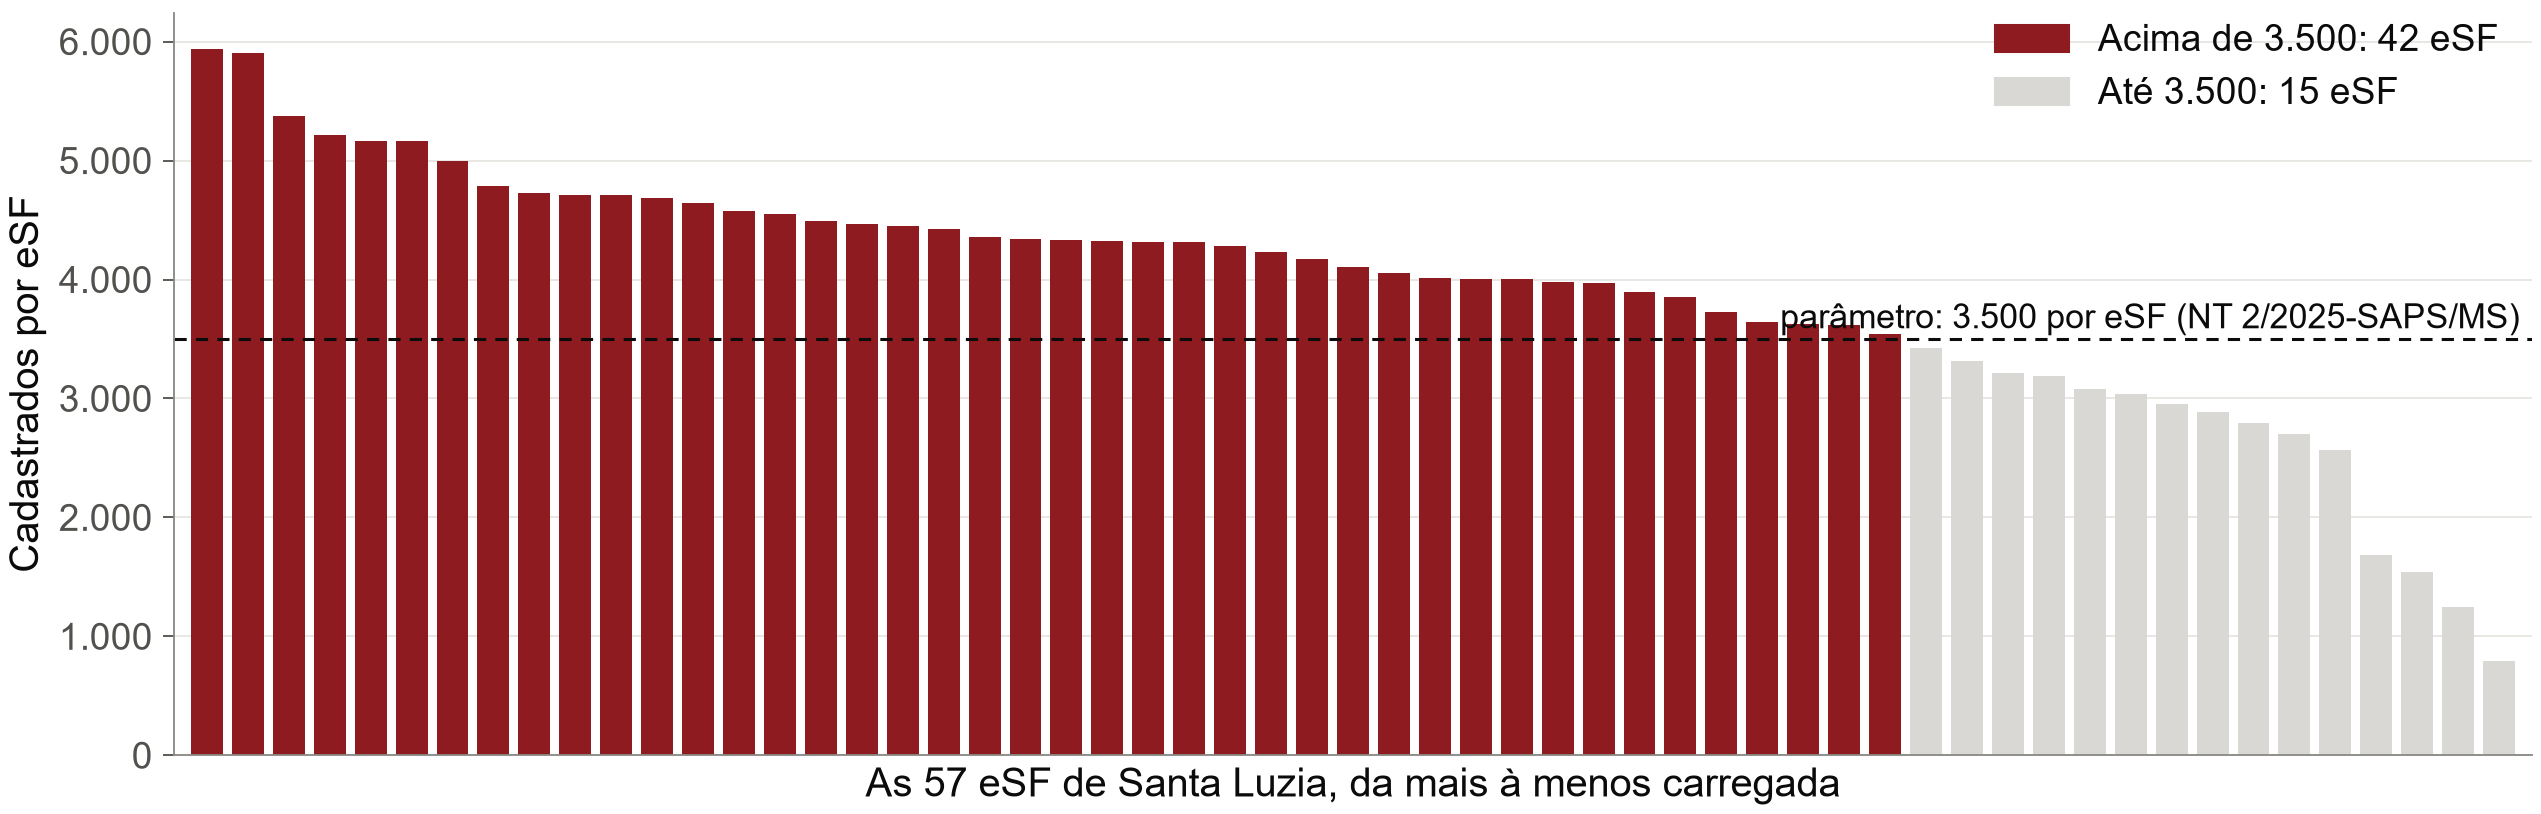
\includegraphics[width=0.98\linewidth]{figuras/f02_cadastrados_por_esf.png}
\fonte{Fonte: elaborada pelos autores com dados do e-Gestor APS e do CNES.}
\end{figure}

O déficit de vagas concentra-se em São Benedito, com 0,76 vaga por habitante, contra 1,05 na Sede (Figura \ref{fig:f03}).

\begin{figure}[!htb]
\centering
\caption{Rede de APS atual e UBS com mais de 3.500 cadastrados por eSF}\label{fig:f03}
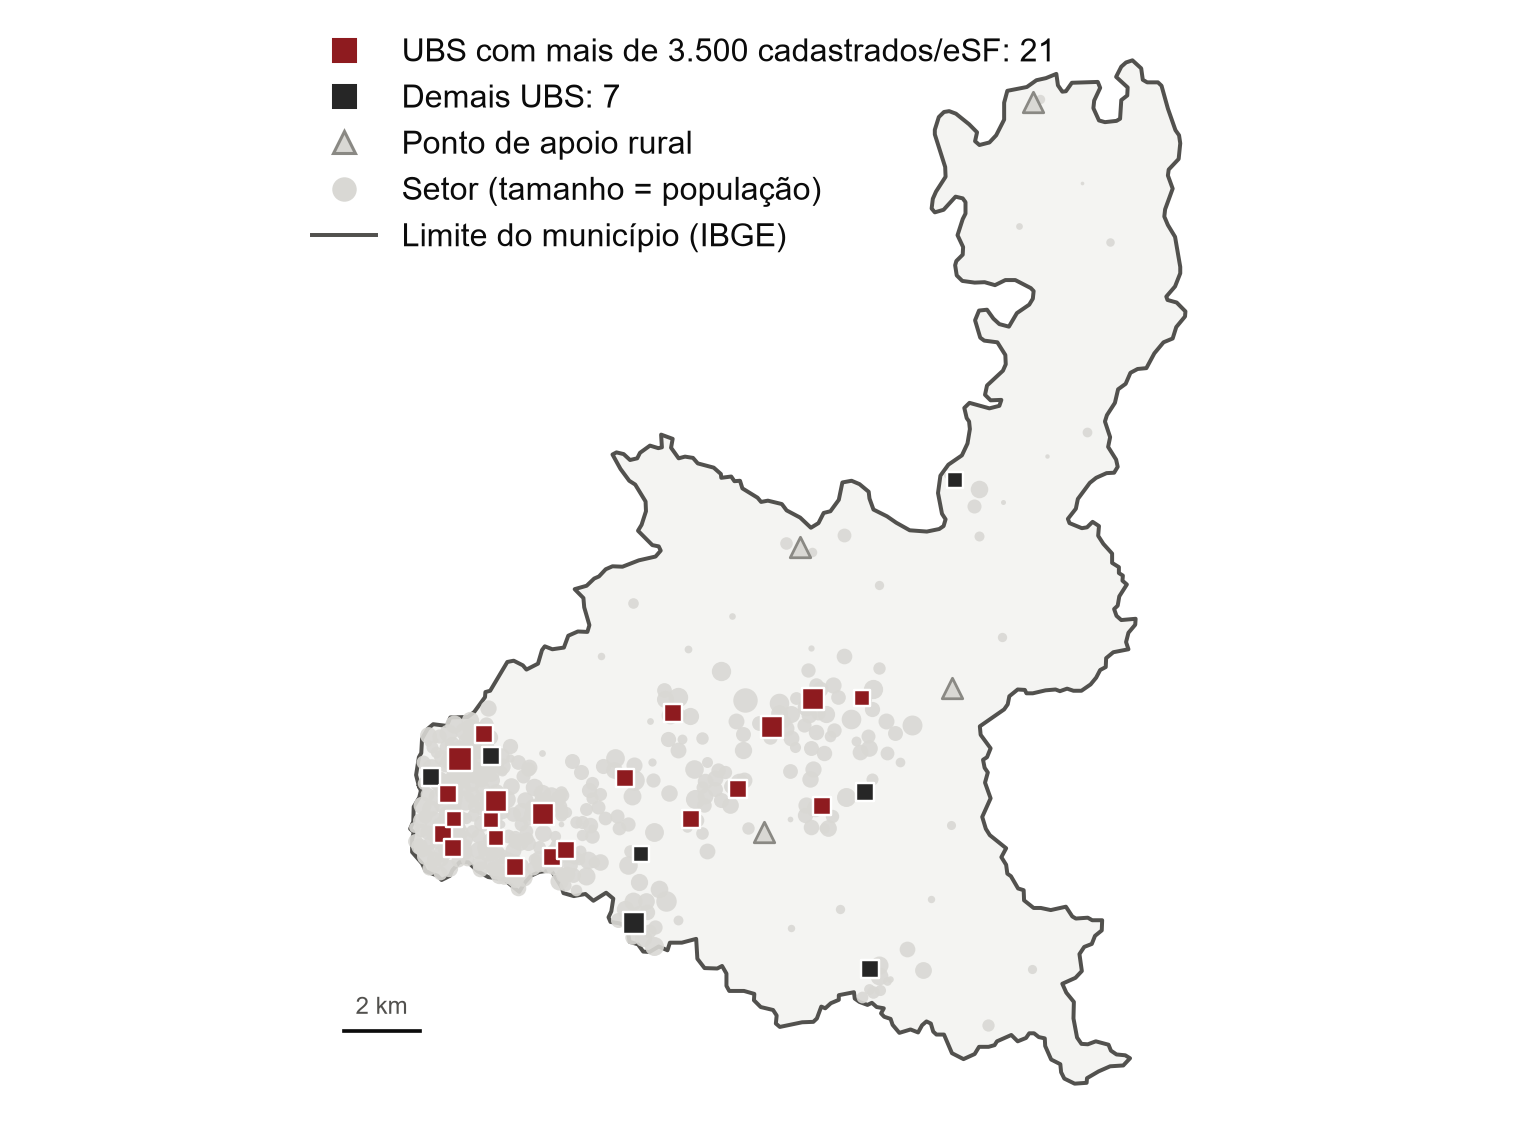
\includegraphics[width=0.89\linewidth]{figuras/f03_mapa_situacao_atual.png}
\fonte{Fonte: elaborada pelos autores com dados do IBGE (2023), do CNES e do e-Gestor APS.}
\end{figure}

\subsection{Comparação dos cenários do modelo base}\label{sec:4.2}

A Tabela \ref{tab:comp} e a Figura \ref{fig:f07} comparam os cenários, e a Figura \ref{fig:f05} mostra onde ficam as eSF novas em cada um. Todas as soluções foram conferidas pela verificação independente; a última linha informa o gap de otimalidade de cada etapa.

\begin{table}[!htb]
\centering
\small
\caption{Comparação dos cenários}\label{tab:comp}
\begin{tabular}{@{}L{\dimexpr 0.3606\linewidth-2\tabcolsep\relax}C{\dimexpr 0.1323\linewidth-2\tabcolsep\relax}C{\dimexpr 0.1654\linewidth-2\tabcolsep\relax}C{\dimexpr 0.1654\linewidth-2\tabcolsep\relax}C{\dimexpr 0.1764\linewidth-2\tabcolsep\relax}@{}}
\toprule
\textbf{Indicador} & \textbf{Atual} & \textbf{C1} & \textbf{C2} & \textbf{C3} \\
\midrule
Cobertura geográfica (\%) & 99,3\% & 100,0\% & 100,0\% & 99,3\% \\
Cobertura efetiva pela solução ótima (\%) & 85,21\% & 100,00\% & 100,00\% & 99,00\% \\
eSF novas: total (UBS existentes + UBS novas) & – & 16 (9 + 7) & 10 (10 + 0) & 10 (10 + 0) \\
UBS novas (porte) & – & 7 (7 × I) & 0 (–) & 0 (–) \\
Investimento em obras (R\$~mi) & – & 13,92 & 0,00 & 0,00 \\
Custeio líquido anual das eSF novas (R\$~mi) & – & 11,16 & 6,98 & 6,98 \\
eSF volante: população / custo anual (R\$~mi) & – & – & – & 2.302 / 1,04 \\
Esforço anual (\% da despesa com APS) & – & 26,1\% & 12,4\% & 14,3\% \\
Distância média / máxima pela rua (km) & 1,93 / 4,97 & 0,98 / 4,95 & 1,02 / 7,55 & 0,97 / 4,37 \\
Gap das etapas 1 / 2 / 3 & – & 0\% / 0\% / 0,84\% & 10,00\% / 0\% / 0,01\% & 10,00\% / 0\% / 0,01\% \\
\bottomrule
\end{tabular}
\fonte{Fonte: elaborada pelos autores. Esforço anual = custeio líquido das eSF novas + obras em 4 anos (+ eSF volante no C3, sem repasse federal), em \% da despesa com APS em 2025.}
\end{table}

\begin{figure}[!htb]
\centering
\caption{Cobertura, eSF novas, obras e esforço anual por cenário}\label{fig:f07}
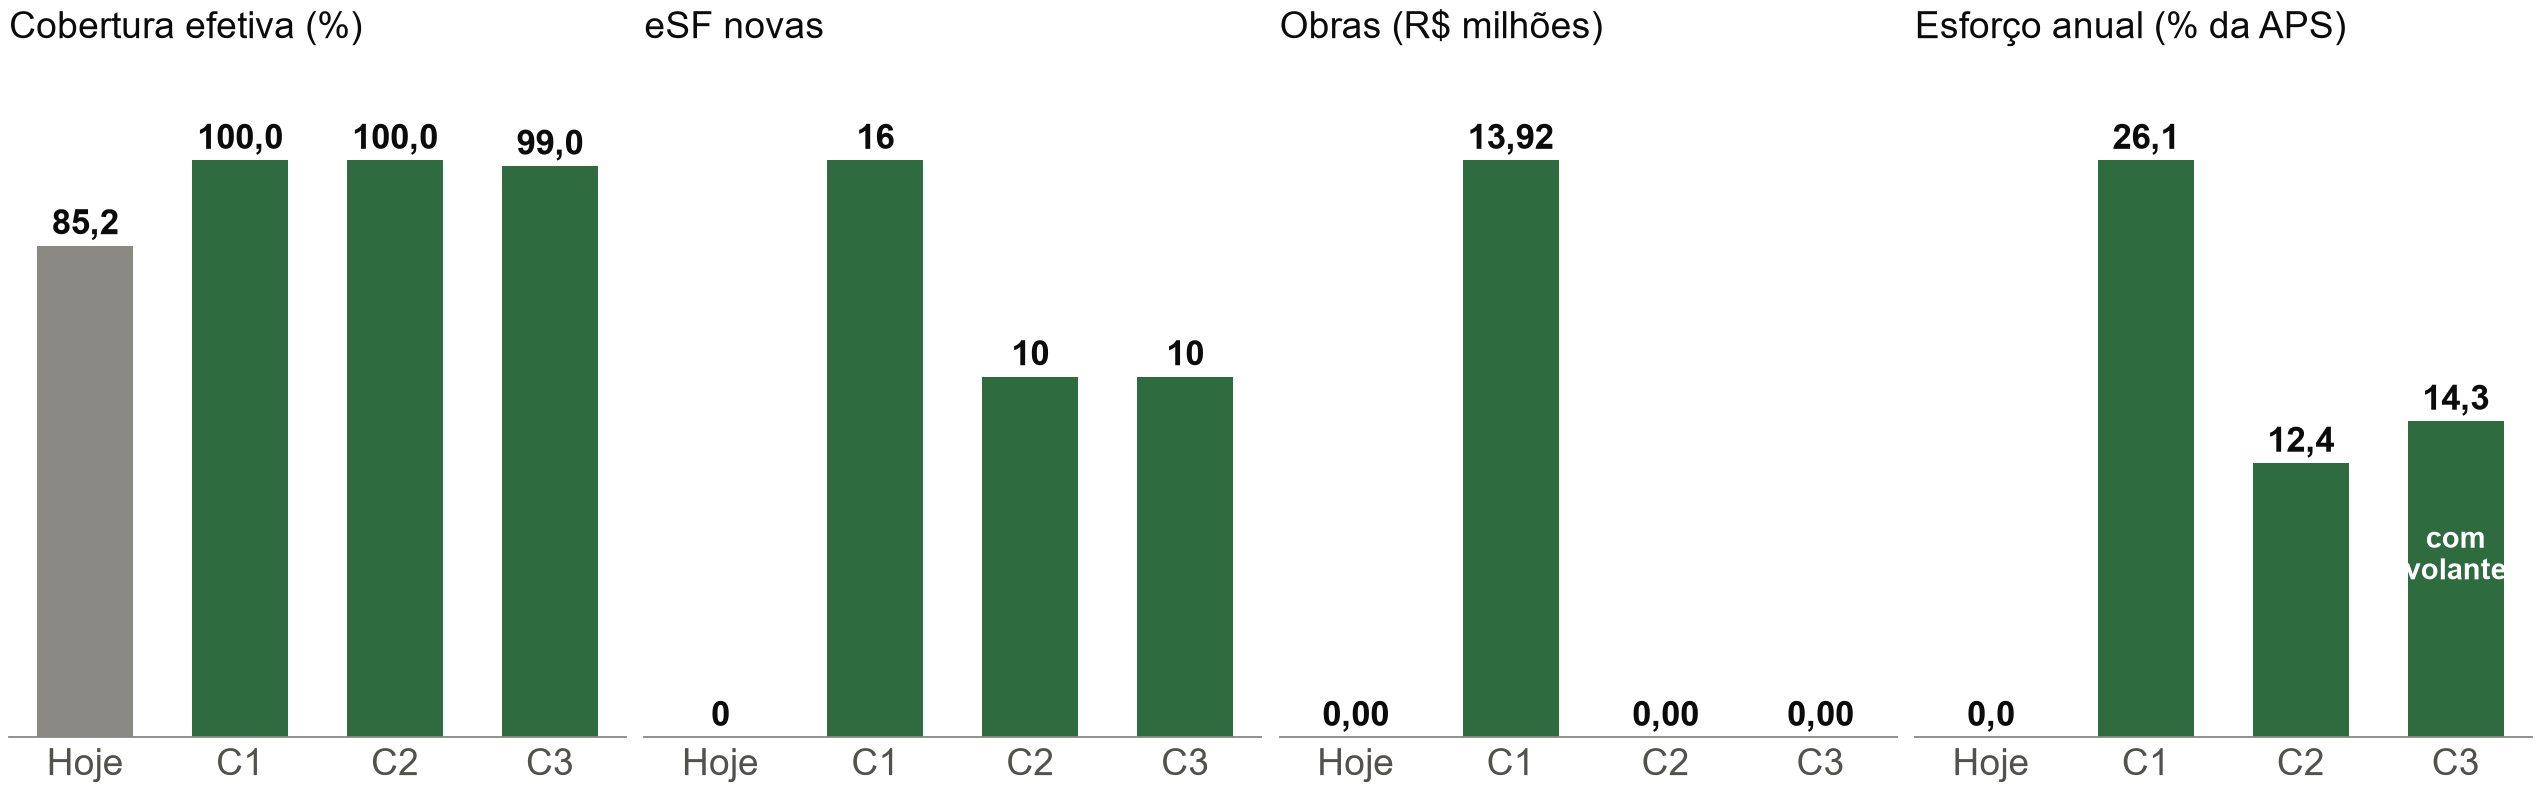
\includegraphics[width=1.00\linewidth]{figuras/f07_comparativo_cenarios.png}
\fonte{Fonte: elaborada pelos autores.}
\end{figure}

\begin{figure}[!htb]
\centering
\caption{eSF novas em cada cenário: UBS existentes que recebem eSF e UBS novas}\label{fig:f05}
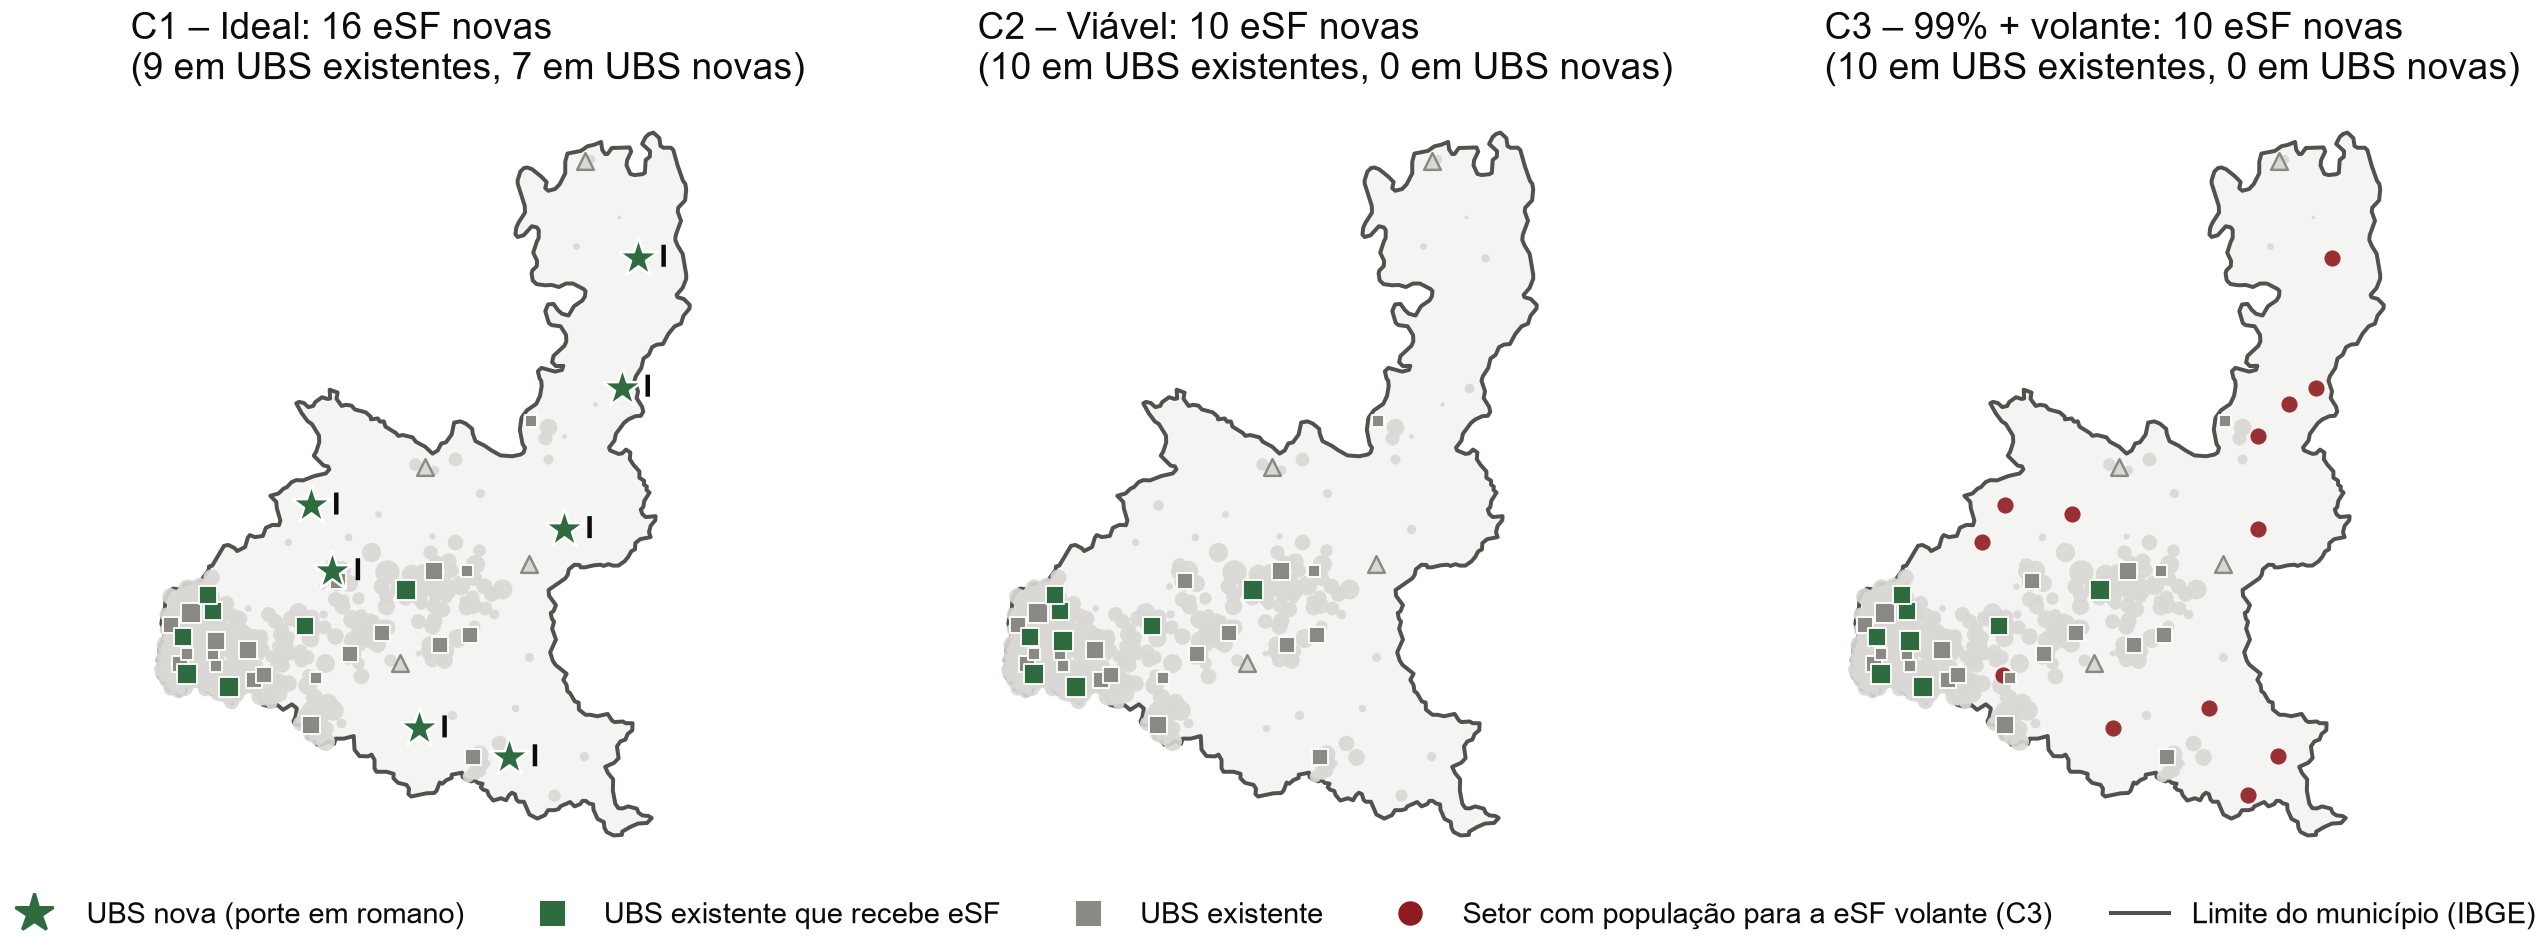
\includegraphics[width=1.00\linewidth]{figuras/f05_mapas_cenarios.png}
\fonte{Fonte: elaborada pelos autores.}
\end{figure}

\subsection{C1 – cenário principal}\label{sec:4.3}

O C1 alcança 100\% de cobertura efetiva com \textbf{16 eSF novas}: 9 em 7 UBS existentes e 7 em 7 UBS novas (7 × I), com investimento de \textbf{R\$~13,92 milhões} em obras e 73 eSF no total. Só pela capacidade, o mínimo seria ⌈(230.382 − 199.500) ÷ 3.500⌉ = 9 eSF; as 7 eSF adicionais decorrem do raio medido pela rua: há comunidades rurais que só alcançam uma unidade a até 5 km se ela for criada perto delas (com setores fracionáveis, o número de eSF seria o mesmo; a indivisibilidade não aumenta o plano). A distância média até a unidade de referência é de 0,98 km pela rua, e a máxima, de 4,95 km. A Tabela \ref{tab:c1} detalha o plano.

\begin{table}[!htb]
\centering
\small
\caption{eSF novas do C1}\label{tab:c1}
\begin{tabular}{@{}L{\dimexpr 0.3826\linewidth-2\tabcolsep\relax}C{\dimexpr 0.1654\linewidth-2\tabcolsep\relax}C{\dimexpr 0.1323\linewidth-2\tabcolsep\relax}C{\dimexpr 0.1323\linewidth-2\tabcolsep\relax}C{\dimexpr 0.1874\linewidth-2\tabcolsep\relax}@{}}
\toprule
\textbf{Unidade} & \textbf{Distrito} & \textbf{eSF atuais} & \textbf{eSF novas} & \textbf{População atendida} \\
\midrule
UBS Duquesa & Sede & 2 & +1 & 10.448 \\
UBS Londrina & São Benedito & 2 & +2 & 13.943 \\
UBS Nova Conquista & São Benedito & 2 & +1 & 10.497 \\
UBS São Cosme & São Benedito & 2 & +1 & 10.401 \\
UBS São Geraldo & Sede & 3 & +1 & 13.776 \\
UBS Tia Lita & São Benedito & 2 & +1 & 10.406 \\
UBS Virgem dos Pobres & São Benedito & 2 & +2 & 13.984 \\
UBS nova, porte I (setor 315780705000156) & Sede & 0 & +1 & 352 \\
UBS nova, porte I (setor 315780705000163) & Sede & 0 & +1 & 307 \\
UBS nova, porte I (setor 315780710000291) & São Benedito & 0 & +1 & 303 \\
UBS nova, porte I (setor 315780705000151) & Sede & 0 & +1 & 233 \\
UBS nova, porte I (setor 315780705000038) & Sede & 0 & +1 & 2.948 \\
UBS nova, porte I (setor 315780705000165) & Sede & 0 & +1 & 148 \\
UBS nova, porte I (setor 315780705000107) & Sede & 0 & +1 & 2.200 \\
\bottomrule
\end{tabular}
\fonte{Fonte: elaborada pelos autores. UBS nova: o local é o centro do setor; o terreno precisa ser verificado.}
\end{table}

A curva de cobertura (Figura \ref{fig:f08}) mostra a maior cobertura efetiva alcançável com cada número de eSF novas, de cerca de 85\% até 100\%. Com setores inteiros, cada ponto exigiria muito tempo de cálculo; a curva foi traçada com setores fracionáveis, uma aproximação (por isso começa em 85,4\%, e não nos 85,2\% de hoje). As primeiras equipes acrescentam até 3.500 pessoas cada; as últimas atendem comunidades rurais pequenas e afastadas, com ganho menor por equipe.

\begin{figure}[!htb]
\centering
\caption{Cobertura efetiva máxima por número de eSF novas (C1)}\label{fig:f08}
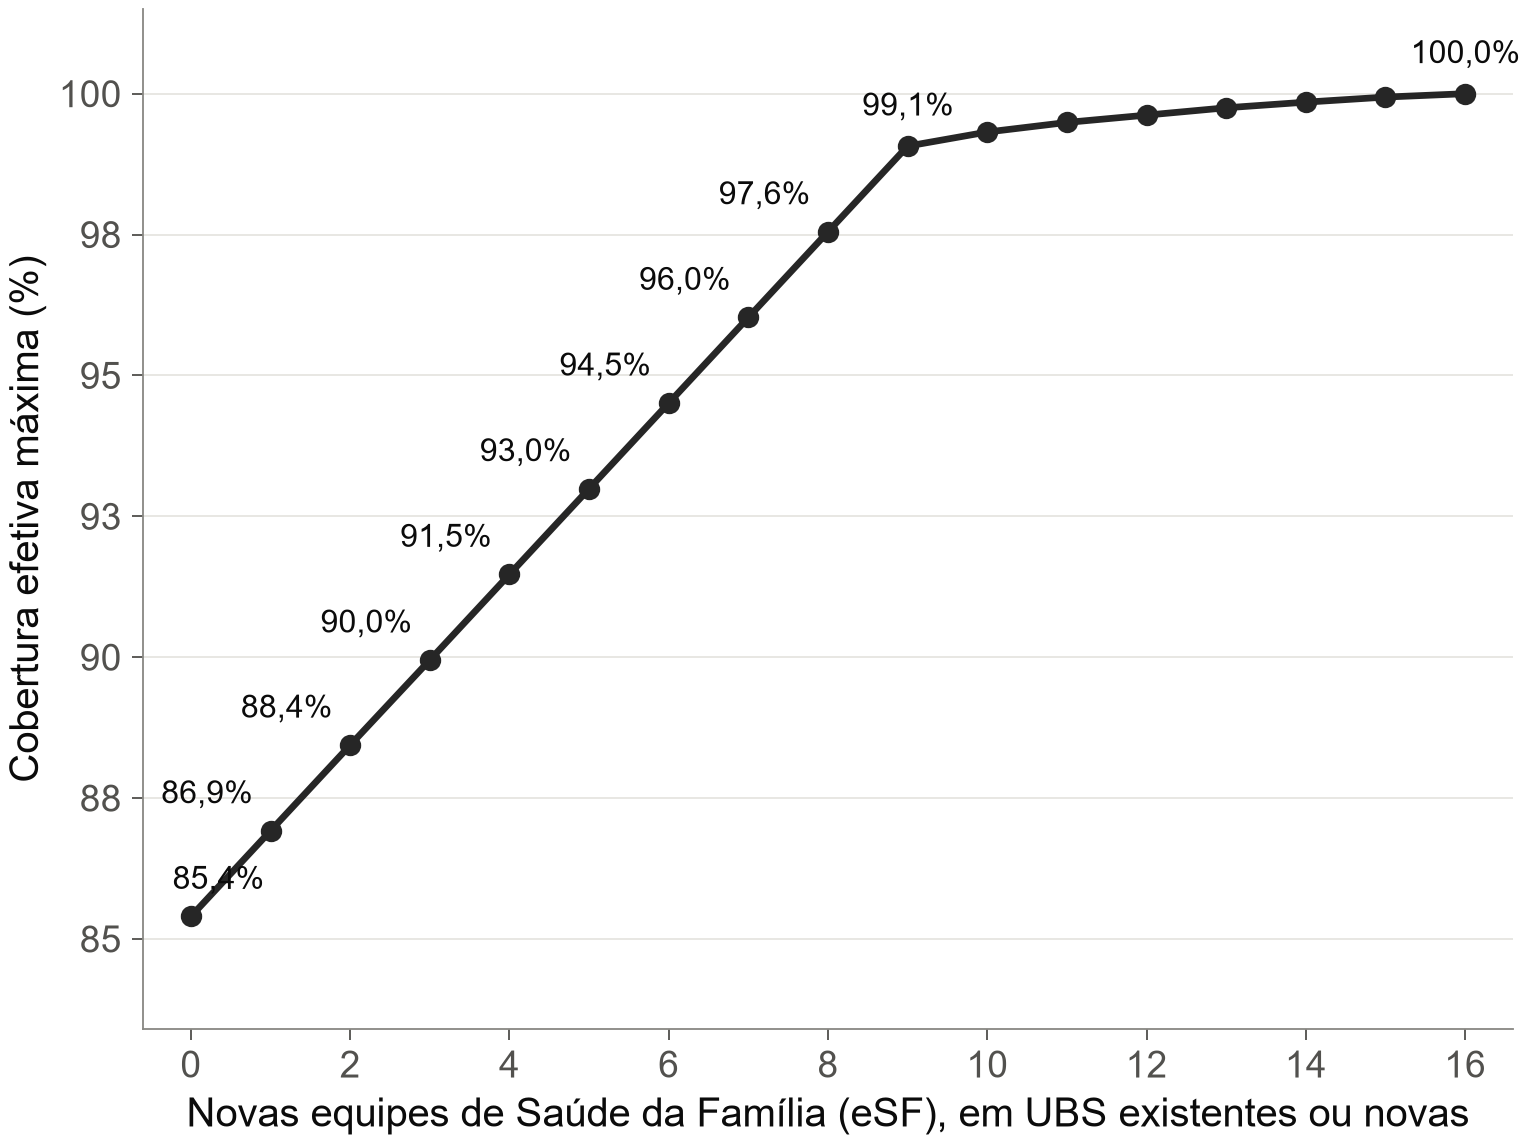
\includegraphics[width=0.89\linewidth]{figuras/f08_curva_C1.png}
\fonte{Fonte: elaborada pelos autores.}
\end{figure}

\subsection{C2 – raios ampliados}\label{sec:4.4}

O C2 exige 10 eSF novas (10 em 8 UBS existentes) e nenhuma obra, contra 16 eSF e R\$~13,92 milhões no C1, com distância média de 1,02 km (a etapa 1 parou no limite de tempo: o limite inferior é de 9 eSF, gap de 10,00\%). Com raios maiores, as comunidades afastadas passam a alcançar unidades existentes, e o plano precisa de menos equipes: a diferença mede o custo de garantir os raios de 3 e 5 km.

\subsection{C3 – 99\% pela solução ótima e eSF volante}\label{sec:4.5}

Com a meta de 99\%, a solução usa 10 eSF novas (10 em 8 UBS existentes), sem obra (o limite inferior é de 9 eSF; gap de 10,00\% na etapa 1) e deixa 2.302 moradores sem cobertura: 2.147 em setores rurais e 155 em setores urbanos, em 13 setores (Tabela \ref{tab:desc}).

\begin{table}[!htb]
\centering
\small
\caption{População sem cobertura na solução ótima do C3}\label{tab:desc}
\begin{tabular}{@{}L{\dimexpr 0.2095\linewidth-2\tabcolsep\relax}C{\dimexpr 0.1323\linewidth-2\tabcolsep\relax}L{\dimexpr 0.2504\linewidth-2\tabcolsep\relax}C{\dimexpr 0.1654\linewidth-2\tabcolsep\relax}L{\dimexpr 0.2425\linewidth-2\tabcolsep\relax}@{}}
\toprule
\textbf{Setor} & \textbf{Distrito} & \textbf{Situação (IBGE)} & \textbf{Pop. sem cobertura} & \textbf{UBS mais próxima (km)} \\
\midrule
315780705000055 & Sede & Área rural exclusive aglomerados & 226 & Bom Destino (6,56) \\
315780705000105 & Sede & Área rural exclusive aglomerados & 146 & Bom Destino (5,04) \\
315780705000147 & Sede & Área rural exclusive aglomerados & 118 & Frimisa (4,76) \\
315780705000151 & Sede & Área rural exclusive aglomerados & 233 & Pinhões (10,04) \\
315780705000156 & Sede & Área rural exclusive aglomerados & 195 & Pinhões (10,36) \\
315780705000162 & Sede & Área rural exclusive aglomerados & 53 & Pinhões (7,55) \\
315780705000163 & Sede & Área não urbanizada de cidade ou vila & 254 & Pinhões (5,57) \\
315780705000165 & Sede & Área rural exclusive aglomerados & 148 & Córrego das Calçadas (7,71) \\
315780705000167 & Sede & Área rural exclusive aglomerados & 404 & Bom Destino (4,97) \\
315780705000170 & Sede & Área rural exclusive aglomerados & 67 & Pinhões (1,72) \\
315780710000165 & São Benedito & Área urbanizada de cidade ou vila & 151 & Frimisa (3,01) \\
315780710000270 & São Benedito & Área urbanizada de cidade ou vila & 4 & Vale das Acácias (0,40) \\
315780710000291 & São Benedito & Área rural exclusive aglomerados & 303 & Frimisa (6,11) \\
\bottomrule
\end{tabular}
\fonte{Fonte: elaborada pelos autores.}
\end{table}

A eSF volante tem como sede a UBS Bom Jesus. Basta uma equipe. A Tabela \ref{tab:rot} e as Figuras \ref{fig:f15} e \ref{fig:f21} mostram o roteiro e o cronograma: 13 pontos, 5.993 km por ano pela rua. O custo anual é de R\$~0,99 milhão de equipe e R\$~54 mil de veículo (entre R\$~23 mil e R\$~57 mil no teste do custo por km), ou R\$~287 por consulta médica esperada. Para visitar cada ponto ao menos uma vez por semana, seriam necessárias 3 equipes, a R\$~3,11 milhões por ano. Comparado ao C1, o C3 usa 6 eSF fixas a menos (5, contando a volante) e R\$~13,92 milhões a menos em obras.

\begin{table}[!htb]
\centering
\small
\caption{Roteiro e demanda da eSF volante (C3)}\label{tab:rot}
\begin{tabular}{@{}L{\dimexpr 0.3165\linewidth-2\tabcolsep\relax}C{\dimexpr 0.1102\linewidth-2\tabcolsep\relax}C{\dimexpr 0.1433\linewidth-2\tabcolsep\relax}C{\dimexpr 0.0992\linewidth-2\tabcolsep\relax}C{\dimexpr 0.1433\linewidth-2\tabcolsep\relax}C{\dimexpr 0.1874\linewidth-2\tabcolsep\relax}@{}}
\toprule
\textbf{Ponto de atendimento} & \textbf{População} & \textbf{Dist. à sede pela rua (km)} & \textbf{Dias por mês} & \textbf{Consultas por dia de visita} & \textbf{Dias do mês} \\
\midrule
Local no setor 315780705000167 & 404 & 12,4 & 3 & 17,7 & 4 11 18 \\
Local no setor 315780710000291 & 303 & 10,9 & 3 & 13,2 & 5 12 19 \\
Local no setor 315780705000163 & 254 & 13,5 & 2 & 16,7 & 9 14 \\
Local no setor 315780705000151 & 233 & 11,1 & 2 & 15,3 & 7 16 \\
Local no setor 315780705000055 & 226 & 12,2 & 2 & 14,8 & 6 17 \\
Local no setor 315780705000156 & 194 & 18,3 & 2 & 12,8 & 8 15 \\
Local no setor 315780710000165 & 151 & 7,9 & 1 & 19,9 & 21 \\
Local no setor 315780705000165 & 148 & 9,7 & 1 & 19,5 & 20 \\
Local no setor 315780705000105 & 146 & 10,0 & 1 & 19,2 & 10 \\
Local no setor 315780705000147 & 118 & 9,6 & 1 & 15,4 & 13 \\
Local no setor 315780705000170 & 67 & 8,8 & 1 & 8,8 & 2 \\
Local no setor 315780705000162 & 53 & 15,5 & 1 & 6,9 & 3 \\
Local no setor 315780710000270 & 4 & 8,0 & 1 & 0,6 & 1 \\
\bottomrule
\end{tabular}
\fonte{Fonte: elaborada pelos autores. Consultas: 1,575 consulta médica básica por habitante por ano (BRASIL, 2002; portaria revogada, usada como ordem de grandeza).}
\end{table}

\begin{figure}[!htb]
\centering
\caption{eSF volante do C3: sede, pontos de atendimento e setores atendidos}\label{fig:f15}
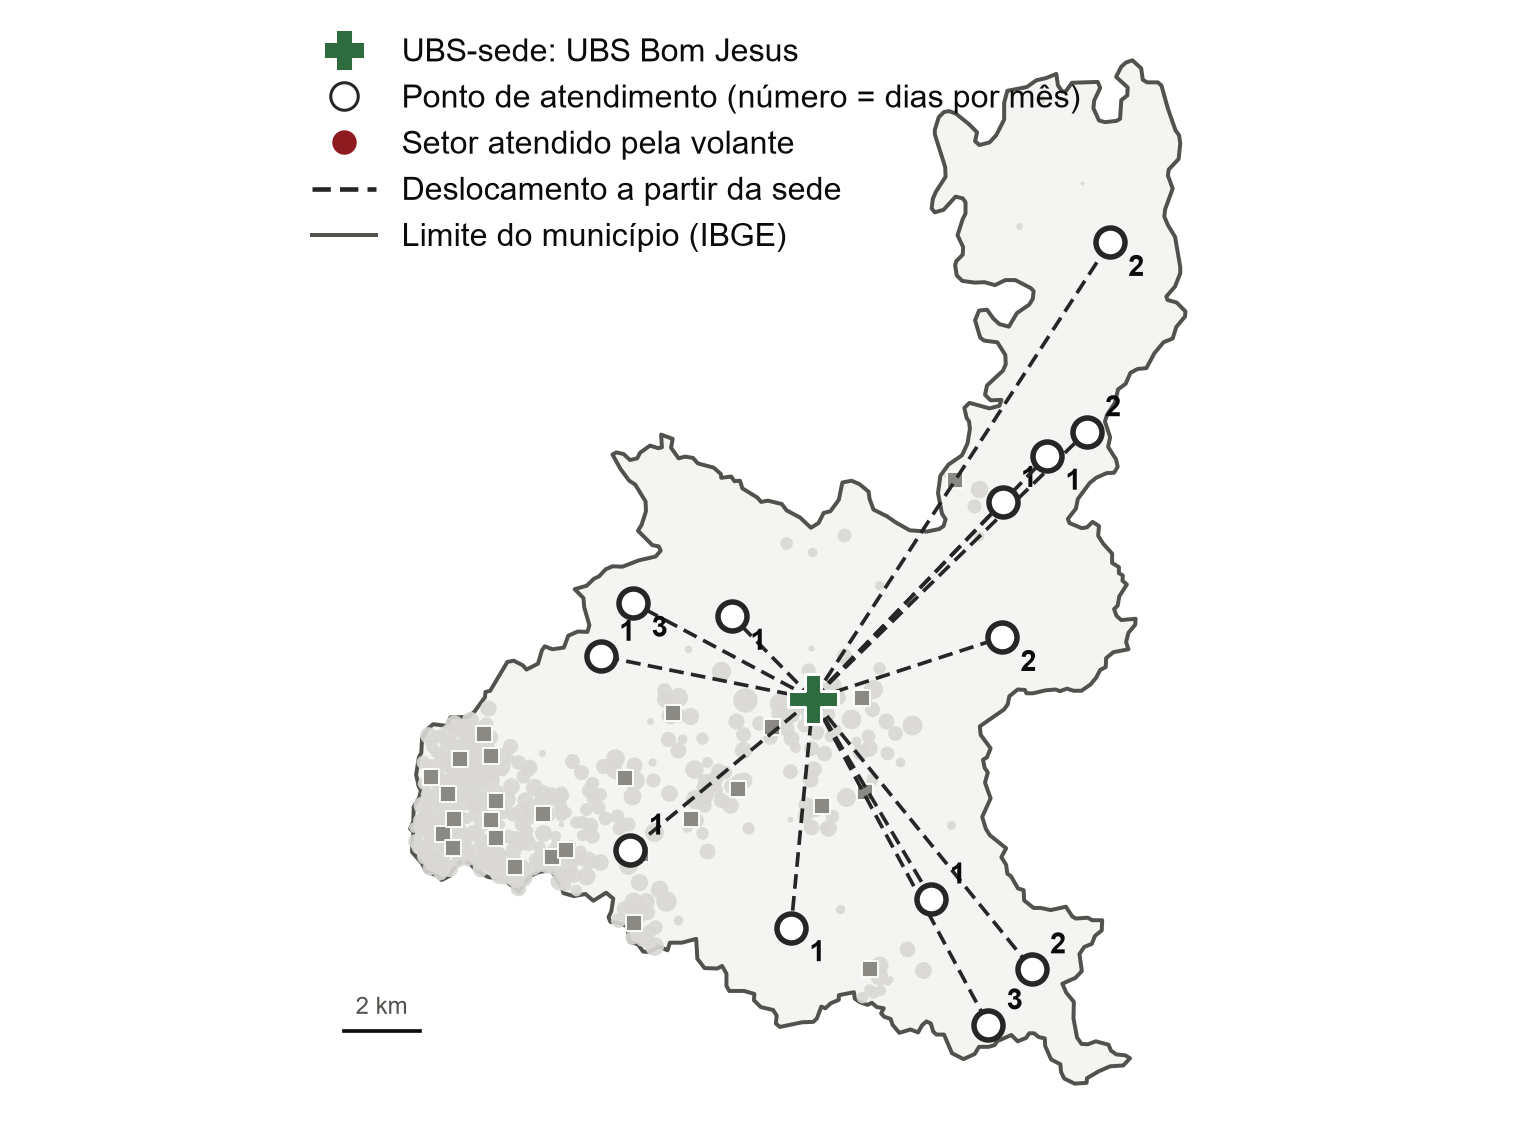
\includegraphics[width=0.89\linewidth]{figuras/f15_volante.png}
\fonte{Fonte: elaborada pelos autores.}
\end{figure}

\begin{figure}[!htb]
\centering
\caption{Cronograma mensal da eSF volante (dia útil e ponto atendido)}\label{fig:f21}
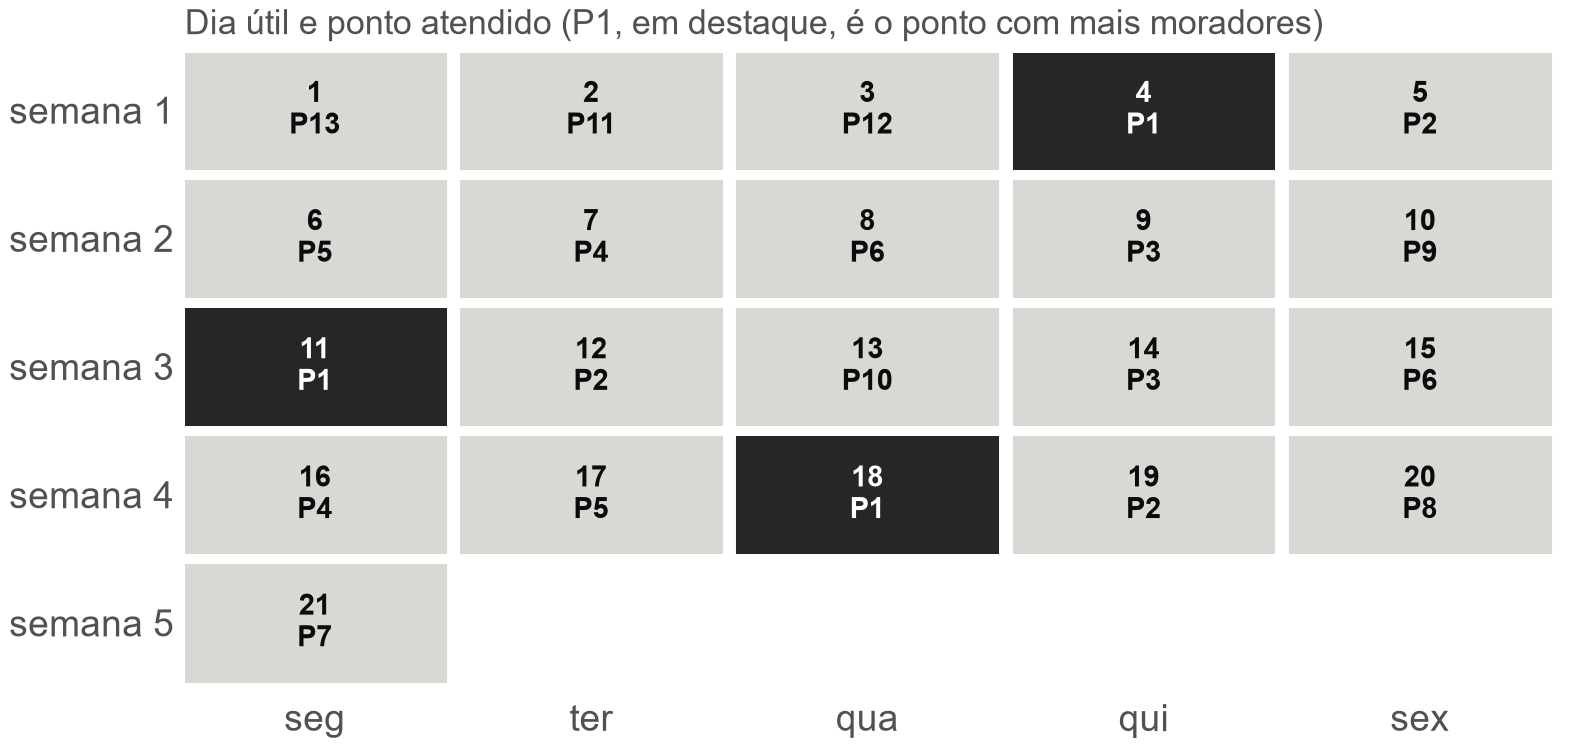
\includegraphics[width=0.89\linewidth]{figuras/f21_cronograma_volante.png}
\fonte{Fonte: elaborada pelos autores.}
\end{figure}

\subsection{Modelo base × modelo integrado}\label{sec:4.6}

A Tabela \ref{tab:int} compara, com os mesmos preços, a solução do modelo base (C1) e a do modelo integrado (custo anual total em reais). O modelo integrado escolhe o mesmo número de eSF novas (16), com 7 UBS novas, contra 7. O custo total anual é de R\$~18,83 milhões no integrado e de R\$~18,83 milhões no modelo base: com os preços de referência, os dois modelos chegam ao mesmo plano. O custeio das eSF domina o custo do governo; o deslocamento é um custo da população, da ordem de R\$~2,5 milhões por ano, e varia pouco entre os planos (Figura \ref{fig:f19}).

\begin{table}[!htb]
\centering
\small
\caption{Custo anual do C1 no modelo base e no modelo integrado (R\$~milhões de 2025)}\label{tab:int}
\begin{tabular}{@{}L{\dimexpr 0.3937\linewidth-2\tabcolsep\relax}C{\dimexpr 0.3032\linewidth-2\tabcolsep\relax}C{\dimexpr 0.3032\linewidth-2\tabcolsep\relax}@{}}
\toprule
\textbf{Parcela} & \textbf{Modelo base (lexicográfico)} & \textbf{Modelo integrado} \\
\midrule
eSF novas (governo) & 15,77 & 15,77 \\
Obras anualizadas (governo) & 0,56 & 0,56 \\
\textbf{Governo, total} & \textbf{16,33} & \textbf{16,33} \\
Deslocamento (população) & 2,50 & 2,50 \\
\textbf{Custo total} & \textbf{18,83} & \textbf{18,83} \\
eSF novas / UBS novas & 16 / 7 & 16 / 7 \\
Distância média pela rua (km) & 0,98 & 0,98 \\
Gap & 0,84\% & 0,16\% \\
\bottomrule
\end{tabular}
\fonte{Fonte: elaborada pelos autores. $C_{\mathrm{eSF}}$ = R\$~986 mil; V = 25 anos; $C_{\mathrm{desl}}$ = R\$~11,07 por pessoa × km por ano.}
\end{table}

\begin{figure}[!htb]
\centering
\caption{Custo anual por parcela: modelo base e modelo integrado}\label{fig:f19}
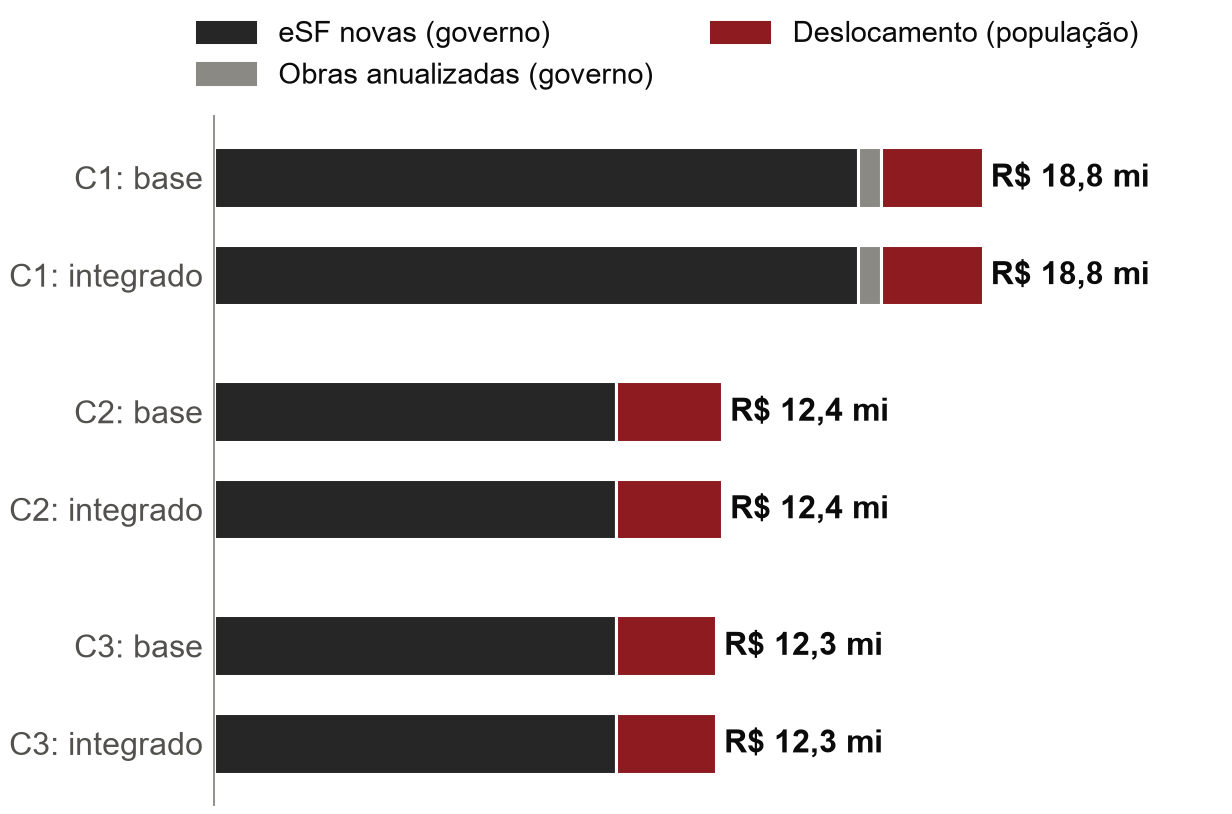
\includegraphics[width=0.89\linewidth]{figuras/f19_integrado.png}
\fonte{Fonte: elaborada pelos autores.}
\end{figure}

A Figura \ref{fig:f20} mostra o efeito do valor do deslocamento. A solução integrada muda a partir de 2 vezes o valor de referência, quando passa a ter 16 eSF novas e 10 UBS novas, com distância média de 0,92 km. Com vida útil de 10 anos, o integrado escolhe 16 eSF e 7 UBS novas. No C2, o integrado escolhe 10 eSF e nenhuma UBS nova, contra 10 e 0 no modelo base (solução no limite de tempo, gap de 7,33\%; a igualdade não está provada). No C3, o integrado escolhe 10 eSF e nenhuma UBS nova, contra 10 e 0 no modelo base (solução no limite de tempo, gap de 7,98\%; a igualdade não está provada). Nas rodadas com 2, 5, 10 e 20 vezes o valor de referência, o solver parou no limite de tempo, com gap de 0,48\%, 1,49\%, 2,43\% e 0,87\%, respectivamente: os planos são viáveis e verificados, mas pode haver plano um pouco mais barato. A comparação indica que a ordem de prioridade do modelo base, primeiro as equipes e depois a obra e a distância, é coerente com a magnitude dos custos em reais: uma eSF custa cerca de R\$~1 milhão por ano, valor que só seria compensado por uma redução muito grande do deslocamento.

\begin{figure}[!htb]
\centering
\caption{Modelo integrado: plano escolhido e distância média por valor do custo de deslocamento}\label{fig:f20}
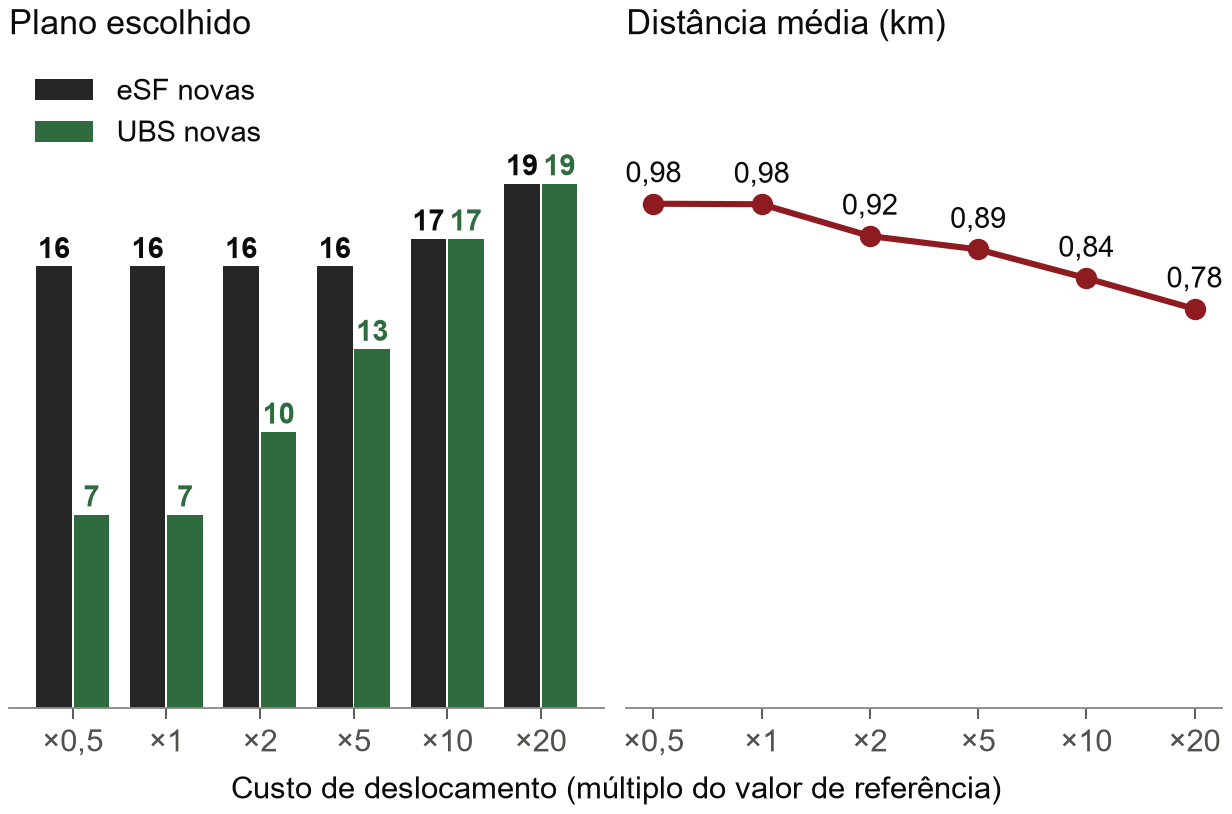
\includegraphics[width=0.89\linewidth]{figuras/f20_integrado_deslocamento.png}
\fonte{Fonte: elaborada pelos autores.}
\end{figure}

\subsection{Análise de sensibilidade}\label{sec:4.7}

A Tabela \ref{tab:sens} e a Figura \ref{fig:f09} mostram o efeito de alterar uma premissa do C1 de cada vez.

\begin{table}[!htb]
\centering
\small
\caption{Sensibilidade do cenário principal (C1)}\label{tab:sens}
\begin{tabular}{@{}L{\dimexpr 0.2724\linewidth-2\tabcolsep\relax}C{\dimexpr 0.0992\linewidth-2\tabcolsep\relax}C{\dimexpr 0.1543\linewidth-2\tabcolsep\relax}C{\dimexpr 0.0882\linewidth-2\tabcolsep\relax}C{\dimexpr 0.1102\linewidth-2\tabcolsep\relax}C{\dimexpr 0.1102\linewidth-2\tabcolsep\relax}C{\dimexpr 0.1654\linewidth-2\tabcolsep\relax}@{}}
\toprule
\textbf{Cenário} & \textbf{Cob. atual} & \textbf{eSF novas (exist. + novas)} & \textbf{UBS novas} & \textbf{Obras (R\$~mi)} & \textbf{Dist. média (km)} & \textbf{Gap 1 / 2 / 3} \\
\midrule
\textbf{C1 – Ideal (cenário principal)} & \textbf{85,2\%} & \textbf{16 (9 + 7)} & \textbf{7} & \textbf{13,92} & \textbf{0,98} & \textbf{0\% / 0\% / 0,84\%} \\
3.000 pessoas por eSF (Portaria nº 3.493/2024) & 73,5\% & 27 (5 + 22) & 18 & 38,00 & 0,84 & 3,70\% / 50,37\% / 42,52\% \\
População do Censo 2022 & 89,4\% & 13 (6 + 7) & 7 & 13,92 & 0,98 & 0\% / 0\% / 0,87\% \\
População projetada para 2029 & 79,9\% & 23 (4 + 19) & 16 & 33,47 & 0,81 & 13,04\% / 57,13\% / 4,78\% \\
Raio urbano de 2 km & 84,8\% & 18 (8 + 10) & 10 & 19,88 & 0,96 & 0\% / 0\% / 0,01\% \\
Raio rural de 3 km & 84,8\% & 23 (8 + 15) & 15 & 29,82 & 0,95 & 0\% / 0\% / 0,80\% \\
Distância em linha reta & 86,4\% & 10 (10 + 0) & 0 & 0,00 & 0,61 & 10,00\% / 0\% / 0,74\% \\
Sem eSF novas nas UBS existentes & 85,2\% & 16 (0 + 16) & 9 & 23,44 & 1,04 & 0\% / 3,22\% / 35,45\% \\
Setor pode ser dividido entre unidades & 85,4\% & 16 (9 + 7) & 7 & 13,92 & 0,97 & 0\% / 0\% / 0\% \\
Com eAP nas UBS novas & 85,2\% & 12,8 (9 + 3,8) & 7 & 13,92 & 0,99 & 3,92\% / 0\% / 1,47\% \\
Candidatos só a mais de 1 km de uma UBS & 85,2\% & 16 (9 + 7) & 7 & 13,92 & 1,01 & 0\% / 0\% / 8,79\% \\
\bottomrule
\end{tabular}
\fonte{Fonte: elaborada pelos autores. Gap > 0: solução viável, verificada, sem prova de otimalidade no limite de tempo.}
\end{table}

\begin{figure}[!htb]
\centering
\caption{eSF novas e investimento em obras por cenário de sensibilidade}\label{fig:f09}
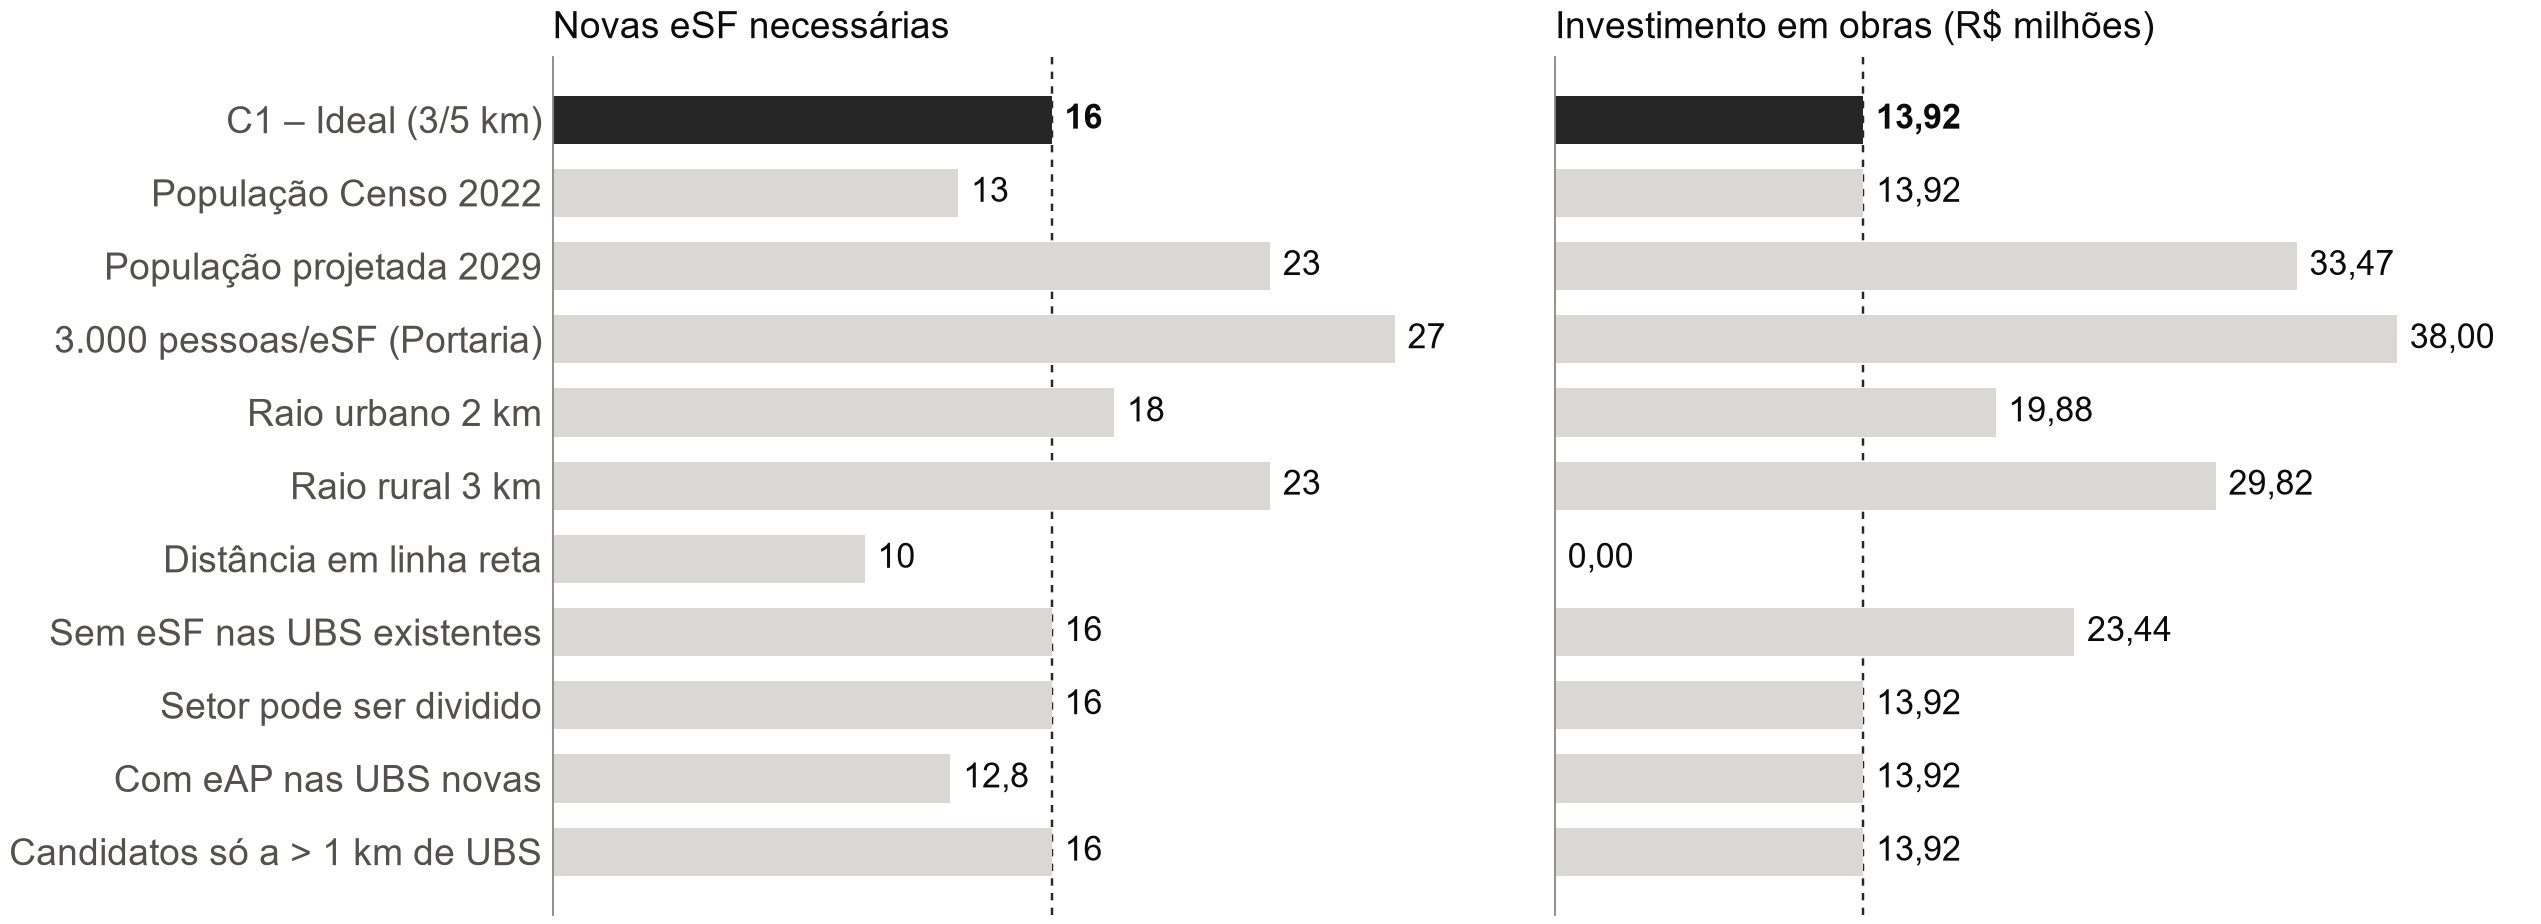
\includegraphics[width=1.00\linewidth]{figuras/f09_sensibilidade.png}
\fonte{Fonte: elaborada pelos autores.}
\end{figure}

Com 3.000 pessoas por eSF, seriam necessárias 27 eSF novas e R\$~38,00 milhões em obras: a capacidade por equipe é a premissa de maior impacto. A população projetada para 2029 exige 23 eSF. Sem eSF novas nas UBS existentes, o plano exigiria 16 eSF em 9 UBS novas e R\$~23,44 milhões em obras: o porte das UBS reduz a obra em R\$~9,52 milhões. Com a distância em linha reta, seriam 10 eSF e nenhuma obra: a medida pela rua aumenta as distâncias e tira comunidades rurais do raio. Se os setores pudessem ser divididos entre unidades, o plano teria as mesmas 16 eSF: a indivisibilidade não aumenta o número de equipes. Reduzir o raio rural para 3 km eleva o plano a 23 eSF. O critério alternativo de candidatos leva a 16 eSF, com distância média de 1,01 km, contra 0,98 km no C1. Nas variantes ``3.000 pessoas por eSF (Portaria nº 3.493/2024)'', ``População projetada para 2029'', ``Distância em linha reta'' e ``Com eAP nas UBS novas'', a etapa 1 parou no limite de tempo: o número de eSF é o de uma solução viável e verificada, e o mínimo pode ser menor (gap na Tabela \ref{tab:sens}).

\subsection{Robustez}\label{sec:4.8}

Com as unidades do C1 fixas (UBS novas e eSF acrescidas), a população de cada setor foi multiplicada por um fator aleatório uniforme de ±10\%, ±20\% e ±30\%, preservando o total do município, em 50 sorteios por nível. Em cada sorteio, um programa inteiro redistribui os setores, inteiros, para maximizar a cobertura efetiva. A cobertura média foi de 99,99\%, 99,99\% e 99,98\%, e o pior sorteio, de 99,85\% (Figura \ref{fig:f10}): com setores indivisíveis e pouca folga de vagas, erros grandes na distribuição da população deixam parte dela sem vaga.

\begin{figure}[!htb]
\centering
\caption{Cobertura efetiva do C1 com erros aleatórios na população dos setores}\label{fig:f10}
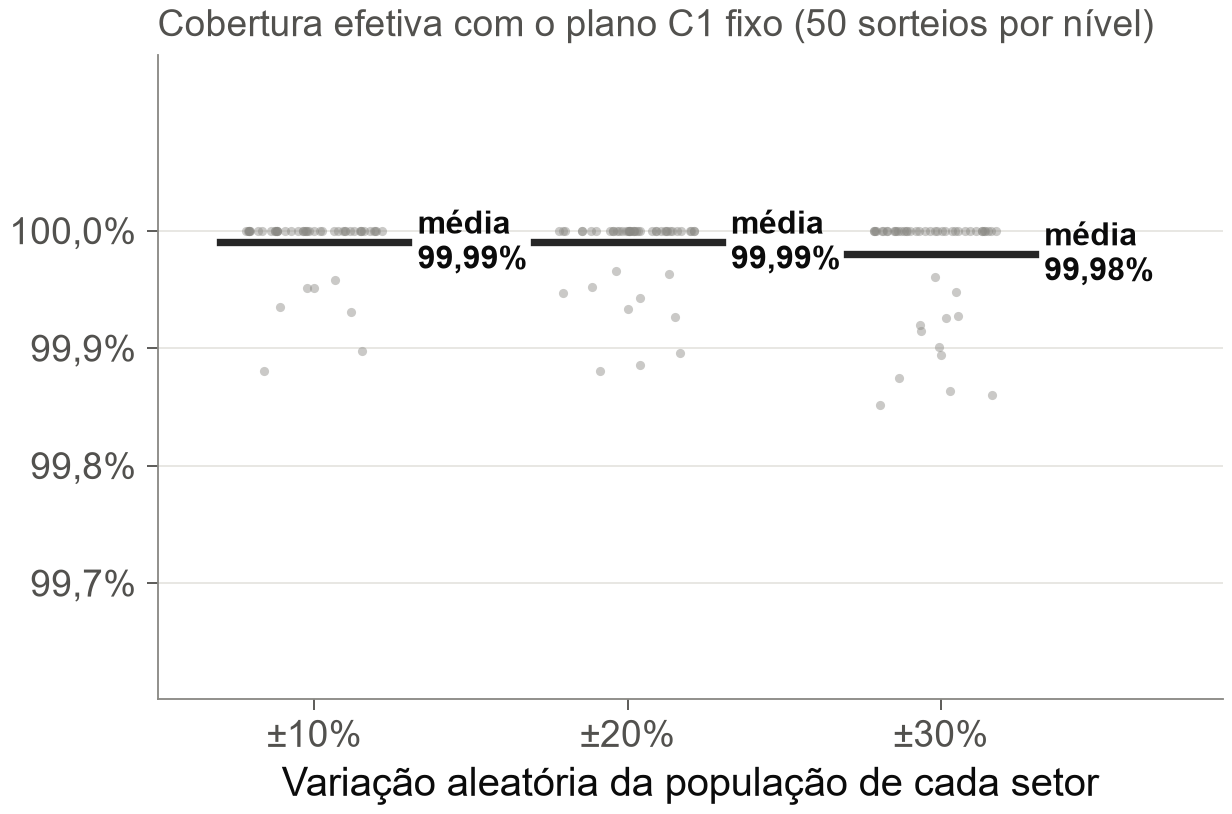
\includegraphics[width=0.83\linewidth]{figuras/f10_estresse_demanda.png}
\fonte{Fonte: elaborada pelos autores.}
\end{figure}

Mantida a taxa anual de crescimento observada entre o Censo 2022 e a estimativa de 2025, o plano C1 cobriria 94,7\% da população em 2029, e o mínimo de eSF novas para 100\% passaria de 16 para no máximo 23 (Figura \ref{fig:f11}); em 2029 o solver parou no limite de tempo, com limite inferior de 20 eSF. O plano precisa, portanto, ser revisto periodicamente.

\begin{figure}[!htb]
\centering
\caption{eSF novas mínimas para 100\% de cobertura efetiva, 2025 a 2029}\label{fig:f11}
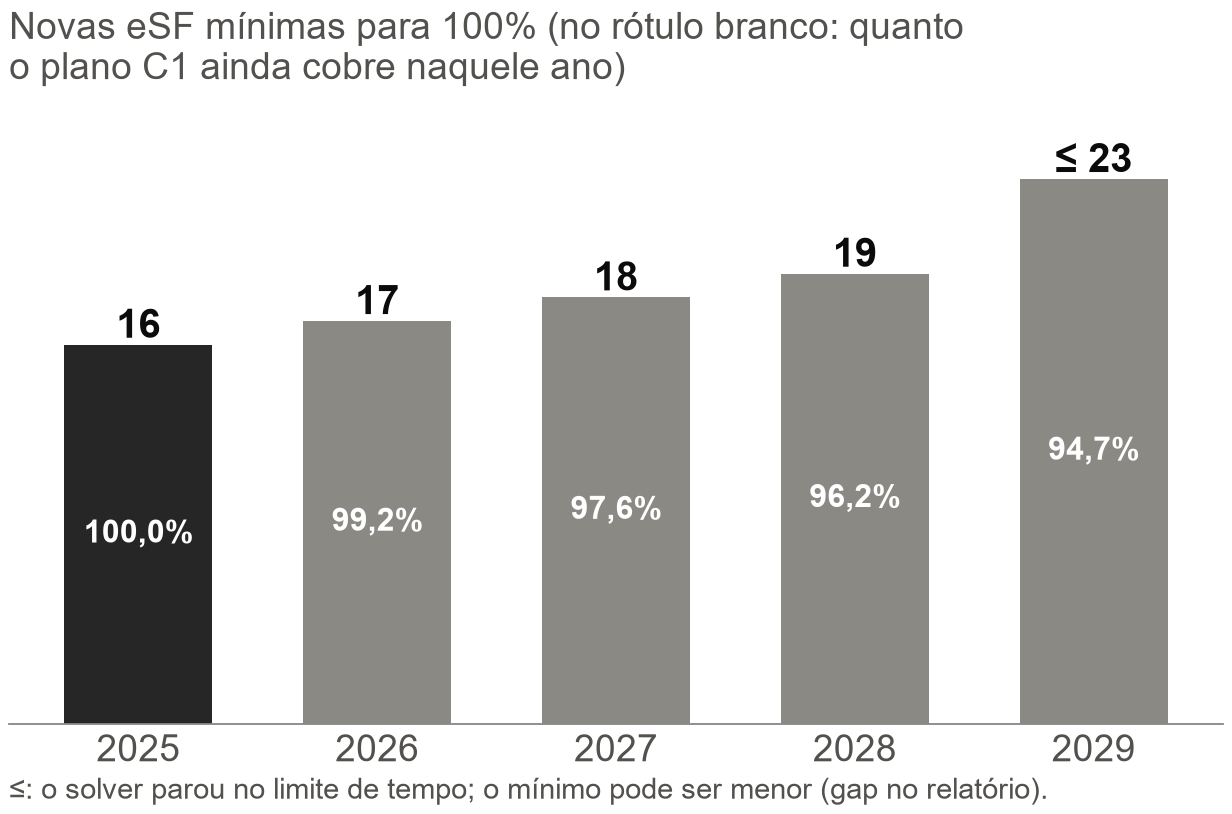
\includegraphics[width=0.83\linewidth]{figuras/f11_crescimento.png}
\fonte{Fonte: elaborada pelos autores.}
\end{figure}

\subsection{Acessibilidade espacial}\label{sec:4.9}

A Tabela \ref{tab:acc} resume as medidas de razão entre oferta e população e de distância, e a Tabela \ref{tab:grav} apresenta o índice gravitacional ajustado nos três valores de $\beta $.

\begin{table}[!htb]
\centering
\small
\caption{Razão oferta/população e distâncias por cenário}\label{tab:acc}
\begin{tabular}{@{}L{\dimexpr 0.4047\linewidth-2\tabcolsep\relax}C{\dimexpr 0.1488\linewidth-2\tabcolsep\relax}C{\dimexpr 0.1488\linewidth-2\tabcolsep\relax}C{\dimexpr 0.1488\linewidth-2\tabcolsep\relax}C{\dimexpr 0.1488\linewidth-2\tabcolsep\relax}@{}}
\toprule
\textbf{Medida} & \textbf{Atual} & \textbf{C1} & \textbf{C2} & \textbf{C3} \\
\midrule
eSF por 1.000 hab. – município & 0,247 & 0,317 & 0,291 & 0,291 \\
Vagas por habitante – Sede & 1,049 & 1,385 & 1,133 & 1,133 \\
Vagas por habitante – São Benedito & 0,762 & 0,952 & 0,952 & 0,952 \\
Distância à unidade mais próxima: média / máx. (km) & 0,96 / 7,55 & 0,91 / 4,95 & 0,96 / 7,55 & 0,96 / 7,55 \\
Distância à unidade de referência: média / máx. (km) & 1,93 / 4,97 & 0,98 / 4,95 & 1,02 / 7,55 & 0,97 / 4,37 \\
\bottomrule
\end{tabular}
\fonte{Fonte: elaborada pelos autores. Distâncias pela rede de ruas; distância à referência: só a população com cobertura efetiva.}
\end{table}

\begin{table}[!htb]
\centering
\small
\caption{Índice gravitacional ajustado (Joseph e Bantock, 1982) por cenário e β}\label{tab:grav}
\begin{tabular}{@{}L{\dimexpr 0.2504\linewidth-2\tabcolsep\relax}C{\dimexpr 0.0661\linewidth-2\tabcolsep\relax}C{\dimexpr 0.1433\linewidth-2\tabcolsep\relax}C{\dimexpr 0.1213\linewidth-2\tabcolsep\relax}C{\dimexpr 0.1213\linewidth-2\tabcolsep\relax}C{\dimexpr 0.1488\linewidth-2\tabcolsep\relax}C{\dimexpr 0.1488\linewidth-2\tabcolsep\relax}@{}}
\toprule
\textbf{Cenário} & \textbf{β} & \textbf{Média ponderada} & \textbf{P10} & \textbf{Mediana} & \textbf{Pop. com A < 0,75 (\%)} & \textbf{Pop. com A < 1 (\%)} \\
\midrule
Situação atual & 1,0 & 0,866 & 0,665 & 0,861 & 25,8\% & 73,0\% \\
Situação atual & 1,5 & 0,866 & 0,501 & 0,791 & 45,7\% & 73,3\% \\
Situação atual & 2,0 & 0,866 & 0,322 & 0,654 & 58,2\% & 76,8\% \\
C1 – Ideal & 1,0 & 1,109 & 0,833 & 1,101 & 5,6\% & 33,5\% \\
C1 – Ideal & 1,5 & 1,109 & 0,658 & 1,027 & 20,6\% & 47,3\% \\
C1 – Ideal & 2,0 & 1,109 & 0,452 & 0,869 & 40,1\% & 61,7\% \\
C2 – Viável & 1,0 & 1,018 & 0,737 & 0,999 & 12,2\% & 50,5\% \\
C2 – Viável & 1,5 & 1,018 & 0,572 & 0,935 & 32,6\% & 56,6\% \\
C2 – Viável & 2,0 & 1,018 & 0,367 & 0,764 & 48,4\% & 64,9\% \\
C3 – 99\% + eSF volante & 1,0 & 1,018 & 0,737 & 0,999 & 12,2\% & 50,5\% \\
C3 – 99\% + eSF volante & 1,5 & 1,018 & 0,572 & 0,935 & 32,6\% & 56,6\% \\
C3 – 99\% + eSF volante & 2,0 & 1,018 & 0,367 & 0,764 & 48,4\% & 64,9\% \\
\bottomrule
\end{tabular}
\fonte{Fonte: elaborada pelos autores. Distância mínima = raio equivalente do setor.}
\end{table}

A média ponderada de $A_{i}$ é igual ao número de vagas por habitante (0,866 hoje e 1,109 no C1), como previsto. O valor de $\beta $ não altera a média, mas muda a dispersão. A ordem dos setores é estável: no C1, a correlação de Spearman entre $\beta $ = 1 e $\beta $ = 2 é de 0,77, e 23 dos 40 setores de menor acessibilidade coincidem. Hoje, 45,7\% da população vive em setores com menos de 0,75 vaga por habitante ($\beta $ = 1,5); com o C1, 20,6\%. Os 40 setores de menor acessibilidade hoje são, em sua maioria, rurais (28 de 40), a 3,26 km pela rua da unidade mais próxima, em média. A melhora do C1 concentra-se em São Benedito, onde as vagas por habitante passam de 0,76 para 0,95 (Figuras \ref{fig:f12} e \ref{fig:f13}).

\begin{figure}[!htb]
\centering
\caption{Distribuição do índice gravitacional ajustado por cenário e β}\label{fig:f12}
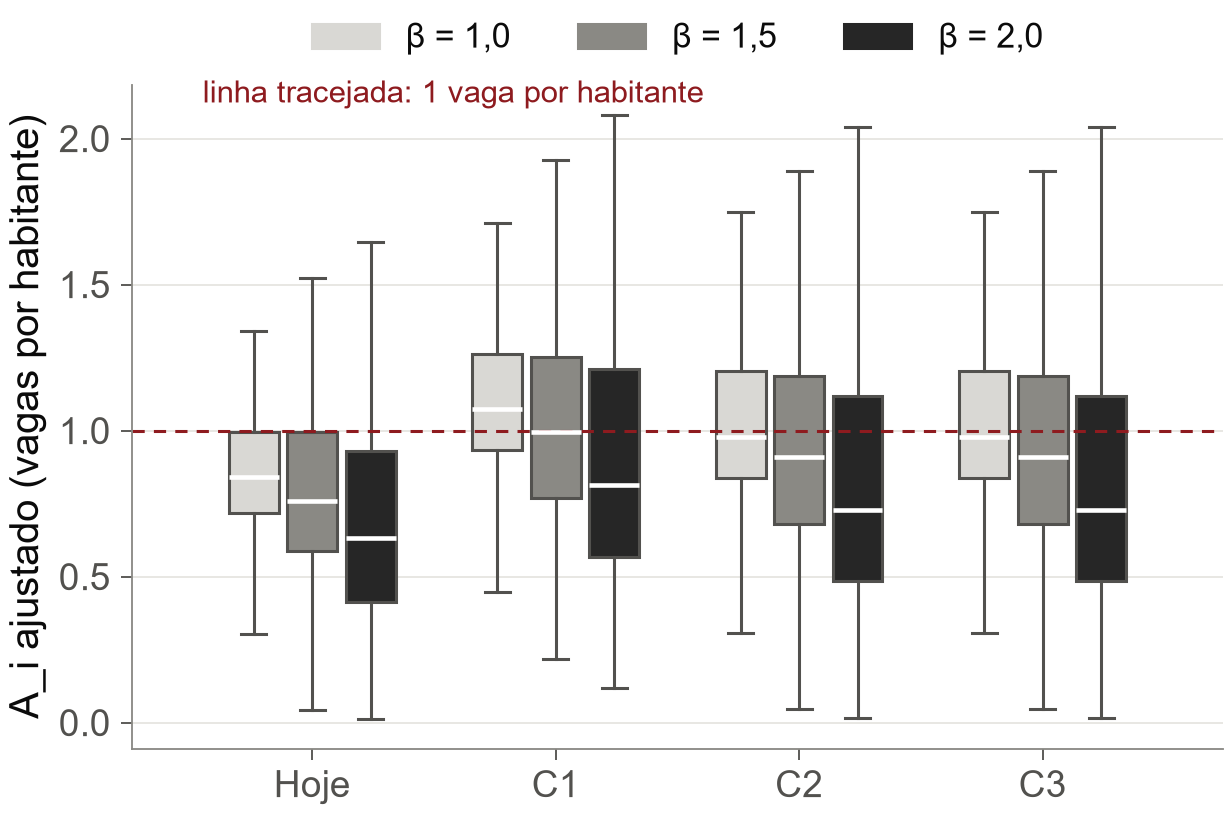
\includegraphics[width=0.83\linewidth]{figuras/f12_acessibilidade_distribuicao.png}
\fonte{Fonte: elaborada pelos autores.}
\end{figure}

\begin{figure}[!htb]
\centering
\caption{Índice gravitacional ajustado por setor, hoje e com o C1 (β = 1,5)}\label{fig:f13}
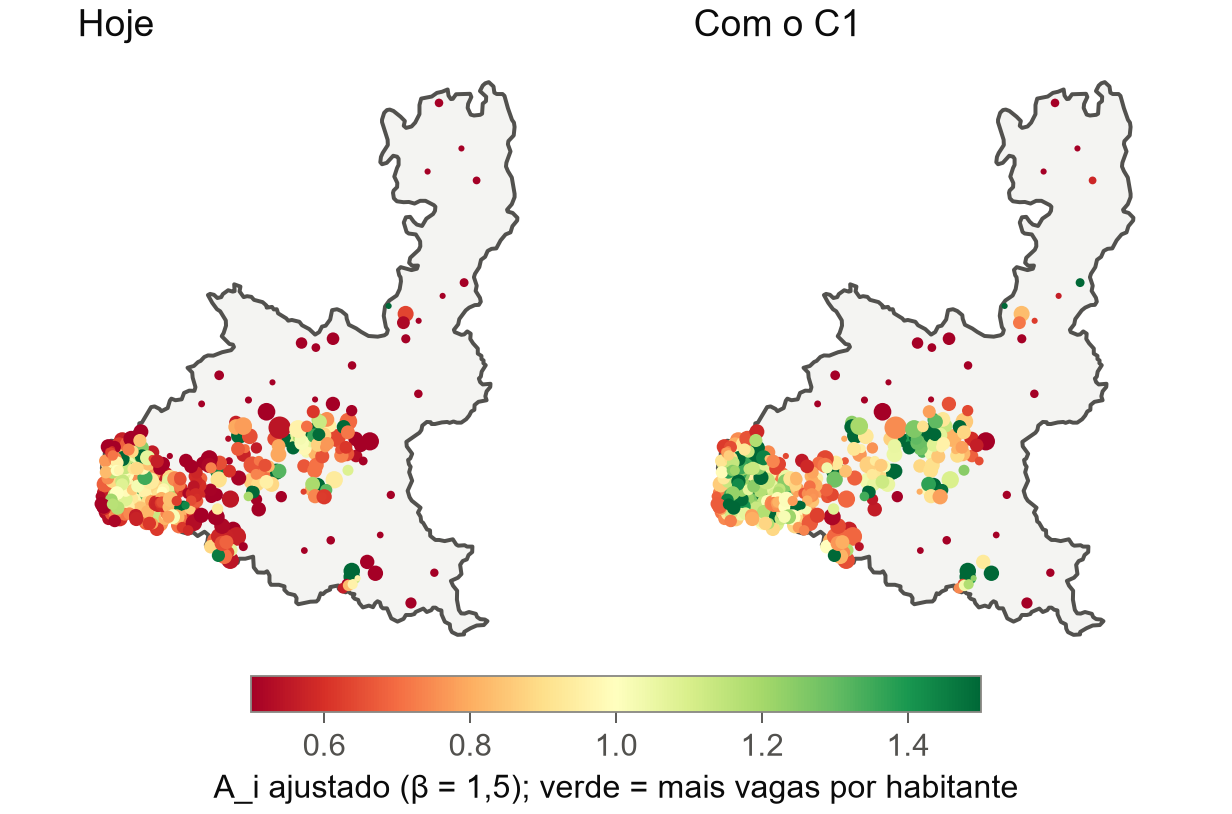
\includegraphics[width=0.89\linewidth]{figuras/f13_mapa_acessibilidade.png}
\fonte{Fonte: elaborada pelos autores.}
\end{figure}

\subsection{Encaminhamentos aos níveis secundário e terciário}\label{sec:4.10}

A Tabela \ref{tab:enc} mostra, para cada tipo de cuidado, as unidades de referência e o acesso da população, pela rede de ruas, na situação atual e no C1; a Figura \ref{fig:f14} resume a parcela da população a mais de 5 km. A matriz completa UBS × serviço e a população referenciada estão no arquivo encaminhamentos.xlsx.

\begin{table}[!htb]
\centering
\small
\caption{Acesso às unidades de referência de média e alta complexidade}\label{tab:enc}
\begin{tabular}{@{}L{\dimexpr 0.1952\linewidth-2\tabcolsep\relax}L{\dimexpr 0.2977\linewidth-2\tabcolsep\relax}C{\dimexpr 0.1984\linewidth-2\tabcolsep\relax}C{\dimexpr 0.1543\linewidth-2\tabcolsep\relax}C{\dimexpr 0.1543\linewidth-2\tabcolsep\relax}@{}}
\toprule
\textbf{Tipo de cuidado} & \textbf{Unidades ativas} & \textbf{Dist. média / máx. (km)} & \textbf{> 5 km (\%)} & \textbf{> 10 km (\%)} \\
\midrule
Urgência & UPA São Benedito & 5,6 / 34,9 (C1: 5,6) & 40,2\% (C1: 40,2\%) & 20,7\% (C1: 20,7\%) \\
Consultas especializadas & Centro de Consultas Especializadas I; Centro de Consultas Especializadas II; CTA; APAE & 3,3 / 27,5 (C1: 3,2) & 15,9\% (C1: 14,6\%) & 3,6\% (C1: 3,6\%) \\
Saúde mental & CAPS Adulto; CAPS Infantojuvenil & 7,3 / 26,0 (C1: 7,3) & 74,0\% (C1: 74,0\%) & 18,7\% (C1: 18,7\%) \\
Saúde bucal especializada & Centro Odontológico Municipal & 7,6 / 25,0 (C1: 7,6) & 73,7\% (C1: 73,7\%) & 30,6\% (C1: 30,6\%) \\
Hospitalar & Hospital Municipal; Hospital São João de Deus & 7,7 / 24,8 (C1: 7,7) & 74,2\% (C1: 74,2\%) & 36,2\% (C1: 36,2\%) \\
\bottomrule
\end{tabular}
\fonte{Fonte: elaborada pelos autores com dados do CNES e do OpenStreetMap. Capacidade não avaliada.}
\end{table}

\begin{figure}[!htb]
\centering
\caption{População a mais de 5 km da unidade de referência, por tipo de cuidado}\label{fig:f14}
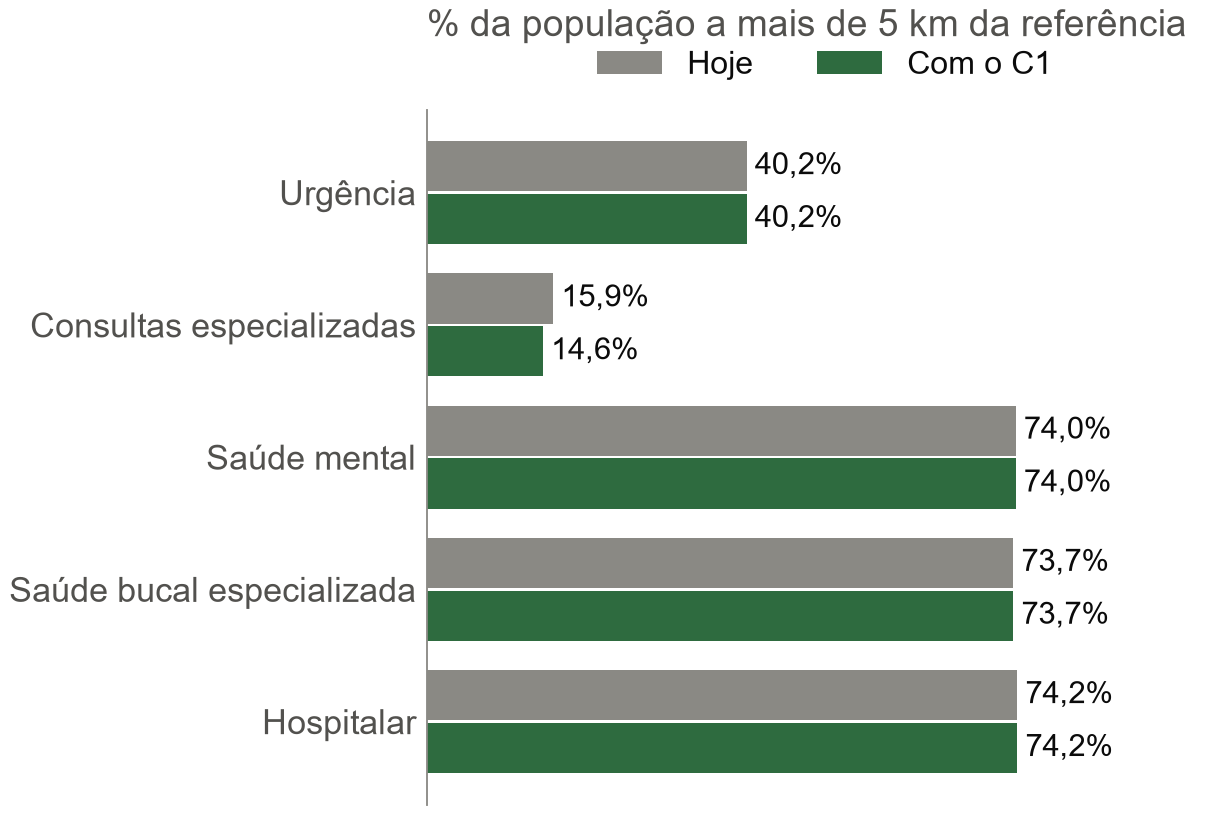
\includegraphics[width=0.83\linewidth]{figuras/f14_encaminhamentos.png}
\fonte{Fonte: elaborada pelos autores.}
\end{figure}

A urgência depende de uma única unidade, a UPA São Benedito; os hospitais e os CAPS ficam na Sede. O critério de proximidade ignora a especialização: o CAPS Infantojuvenil e a APAE, que atendem públicos específicos, aparecem como referência de muitas UBS. Uma regionalização oficial, se disponível, substituiria esse critério.

\subsection{Viabilidade orçamentária}\label{sec:4.11}

No C1, o custeio bruto das 16 eSF novas é de R\$~15,77 milhões por ano; descontado o repasse federal, R\$~11,16 milhões. Com as obras distribuídas em quatro anos, o esforço anual é de \textbf{R\$~14,64 milhões}, 26,1\% da despesa com APS e 7,0\% da despesa total com saúde em 2025 (Tabela \ref{tab:orc} e Figura \ref{fig:f16}). O município aplicou R\$~36,1 milhões acima do mínimo constitucional em 2025.

\begin{table}[!htb]
\centering
\small
\caption{Comparação dos cenários com o orçamento de saúde de 2025 (R\$~milhões por ano)}\label{tab:orc}
\begin{tabular}{@{}L{\dimexpr 0.4378\linewidth-2\tabcolsep\relax}C{\dimexpr 0.1874\linewidth-2\tabcolsep\relax}C{\dimexpr 0.1874\linewidth-2\tabcolsep\relax}C{\dimexpr 0.1874\linewidth-2\tabcolsep\relax}@{}}
\toprule
\textbf{Item} & \textbf{C1} & \textbf{C2} & \textbf{C3} \\
\midrule
Custeio bruto das eSF novas & 15,77 & 9,86 & 9,86 \\
(−) Repasse federal adicional & 4,61 & 2,88 & 2,88 \\
(+) Obras por ano (4 anos) & 3,48 & 0,00 & 0,00 \\
(+) eSF volante, sem repasse & – & – & 1,04 \\
\textbf{Esforço anual} & \textbf{14,64} & \textbf{6,98} & \textbf{8,02} \\
\% da despesa com APS em 2025 & 26,1\% & 12,4\% & 14,3\% \\
\bottomrule
\end{tabular}
\fonte{Fonte: elaborada pelos autores com dados do RAG 2025 (SANTA LUZIA, 2026).}
\end{table}

\begin{figure}[!htb]
\centering
\caption{Despesa anual com APS antes e depois de cada cenário}\label{fig:f16}
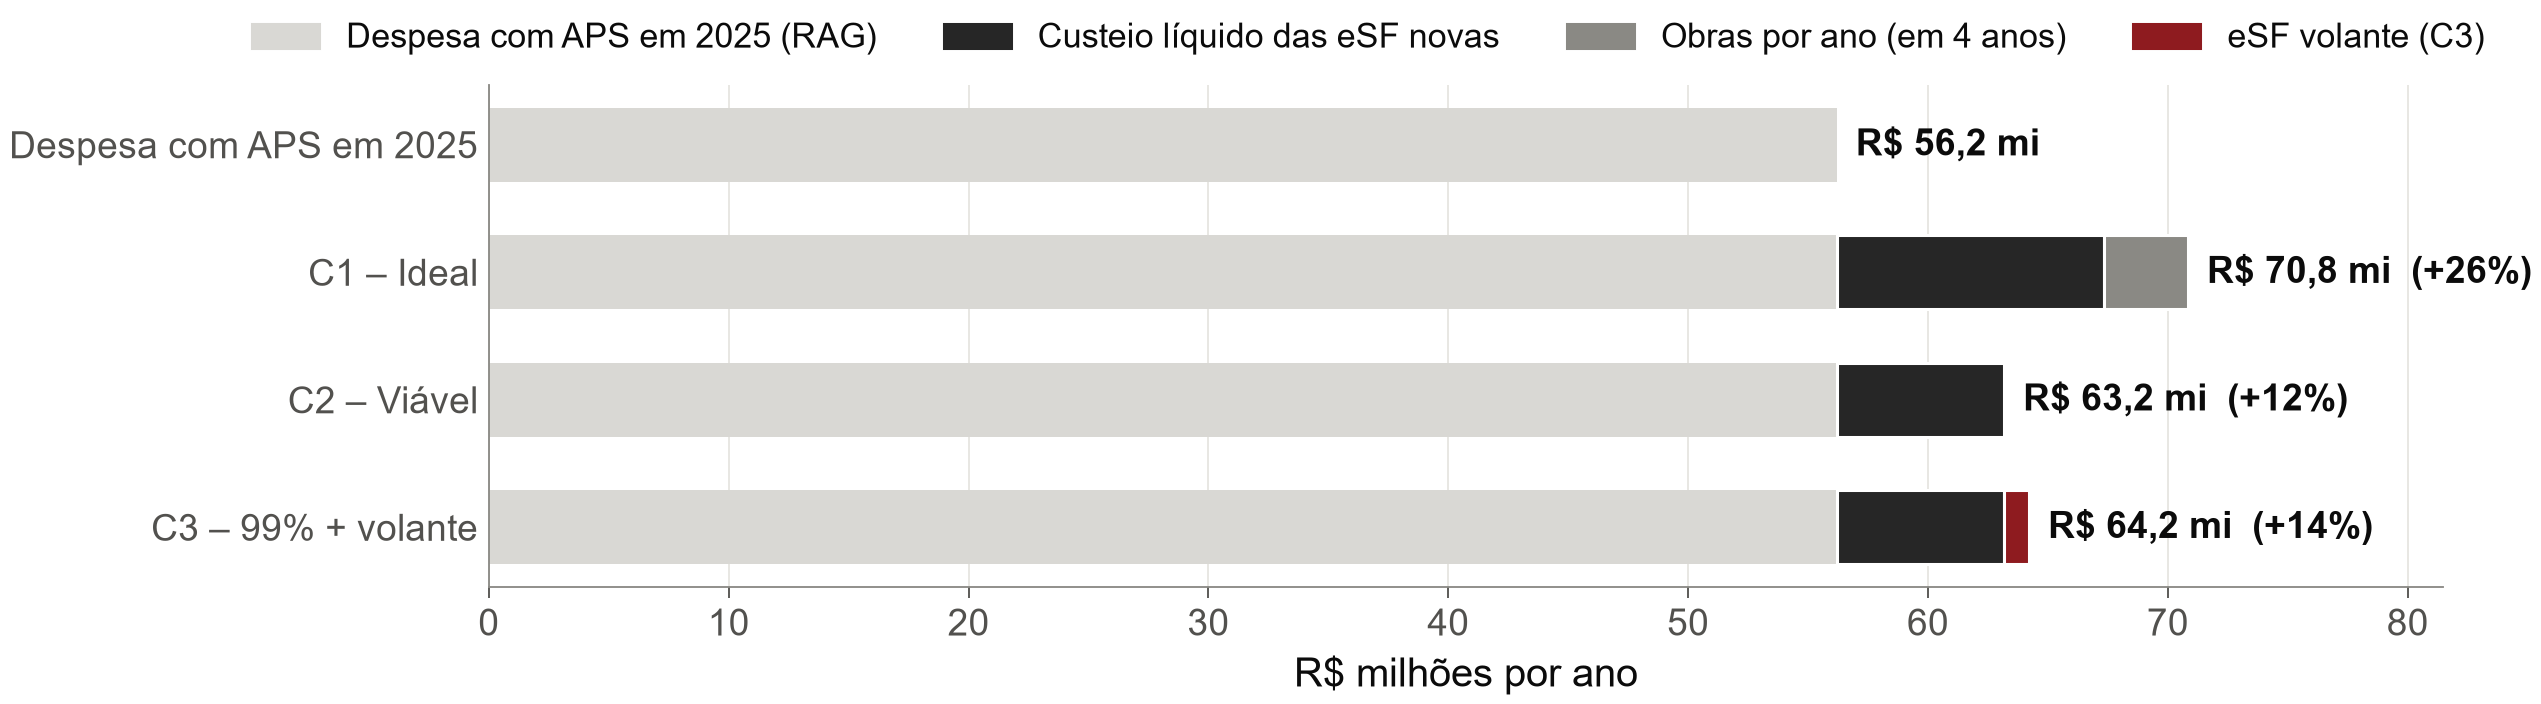
\includegraphics[width=1.00\linewidth]{figuras/f16_orcamento.png}
\fonte{Fonte: elaborada pelos autores com dados do RAG 2025 (SANTA LUZIA, 2026).}
\end{figure}

\subsection{Leitura pela tipologia de necessidade, demanda e oferta}\label{sec:4.12}

Pela tipologia de Santana et al. (2023), os 32.355 moradores que vivem perto de uma UBS lotada estão na situação de necessidade sem oferta suficiente. O C1 elimina essa situação, sobretudo com eSF novas em UBS que têm espaço. No outro extremo, unidades com ocupação baixa seriam oferta com pouca demanda; no C1, a ocupação média é de 90,2\% e a mínima, de 4,2\%, nas unidades criadas para comunidades rurais pequenas, que a eSF volante do C3 poderia atender a outro custo.

\clearpage
\section{Limitações metodológicas}
\begin{enumerate}[label=\alph*),leftmargin=*,itemsep=2pt]
\item A medida de cobertura efetiva corresponde ao acesso potencial (disponibilidade e acessibilidade). Os componentes de utilização ($U$) e de qualidade ($Q$) de Shengelia et al. (2005) não foram medidos: a base não contém produção de atendimentos por equipe nem ganho de saúde por prestador.
\item As distâncias seguem a rede a pé do OpenStreetMap, a partir do centro do setor; a qualidade do mapa, o relevo e a segurança dos trajetos não foram avaliados, e a população do setor é representada por um único ponto.
\item A população de cada setor é a do Censo 2022 ajustada proporcionalmente à estimativa de 2025; erros de distribuição foram avaliados por simulação.
\item O porte das UBS veio de levantamento por CNES, sem dado para UBS Cotegipe; admite-se que acrescentar eSF até o porte não exige obra. Os locais das UBS novas são centros de setor, e os terrenos não foram verificados.
\item O custeio da eSF é aproximado pelo custo médio da APS no município, um teto. O custo de deslocamento do modelo integrado depende de premissas (visitas por ano, renda, caminhada), testadas de 0,5 a 20 vezes o valor de referência; o número de visitas vem de uma portaria já revogada (nº 1.101/2002), usado apenas como ordem de grandeza; o custo por quilômetro da eSF volante usa valores nominais.
\item O coeficiente $\beta $ do índice gravitacional não foi estimado empiricamente; os resultados são apresentados para três valores.
\item A média e a alta complexidade foram avaliadas apenas quanto ao acesso geográfico, com a unidade ativa mais próxima como referência, critério que ignora a especialização de cada serviço; capacidade e pactuações regionais não foram consideradas.
\item O modelo é estático: o crescimento populacional foi tratado por cenários, e não por um modelo multiperíodo.
\item Algumas etapas terminaram no limite de tempo, com solução viável e verificada, mas sem prova de otimalidade; o gap correspondente é informado nas tabelas.
\end{enumerate}


\section{Conclusão}

Com o parâmetro de 3.500 pessoas por eSF e distâncias máximas de 3 km (urbano) e 5 km (rural) pela rede de ruas, 99,3\% da população de Santa Luzia tem uma unidade de APS no raio, mas apenas 85,2\% tem também vaga em uma equipe. O déficit é sobretudo de vagas, concentrado em São Benedito, e, em menor grau, de unidades próximas na zona rural.

O modelo base, de objetivo lexicográfico e com setores indivisíveis, indica que \textbf{16 eSF novas} levam a cidade a 100\% de cobertura efetiva (C1): 9 em 7 UBS existentes e 7 em 7 UBS novas (7 × I), com R\$~13,92 milhões em obras. O porte das UBS existentes permite acomodar a maior parte das equipes sem obra. O esforço anual corresponde a 26,1\% da despesa com APS em 2025. O modelo integrado, que soma em reais o custo do governo e o da população, chega a um plano com o mesmo número de equipes, o que confirma a coerência da ordem de prioridades do modelo base. O resultado mais relevante para a gestão está no último 1\% da população: com a distância pela rua, comunidades rurais pequenas e afastadas só são cobertas por unidades fixas se forem abertas 7 UBS novas, com 7 eSF e R\$~13,92 milhões em obras. O C3 cobre 99\% com 10 eSF nas UBS existentes, sem obra, e atende o restante com uma eSF volante de R\$~1,04 milhão por ano: esforço anual de 14,3\% da despesa com APS, contra 26,1\% no C1. A escolha entre unidades fixas e equipe volante para a zona rural é, portanto, a principal decisão que o modelo coloca para o gestor.

A solução precisa acompanhar o crescimento da cidade e ser revista periodicamente. O acesso à urgência e aos hospitais continua dependente da localização desses serviços, fora do alcance das decisões sobre a rede de APS.


\section*{Declaração de uso de inteligência artificial}

Este trabalho foi elaborado com o apoio de modelos de linguagem de grande escala (LLMs), usados na programação dos modelos e das análises, na organização dos dados e na redação. Os autores revisaram integralmente o conteúdo e assumem total responsabilidade pelas premissas, análises e conclusões apresentadas.

\section*{Disponibilidade de dados e códigos}
Os modelos em GMPL (\texttt{.mod}), os dados (\texttt{.dat} e \texttt{.xlsx}), os códigos em Python e os resultados estão disponíveis em \url{https://github.com/pedroohassen/santa_luzia}.


\section*{Referências}
\bibentrada{ADAY, L. A.; ANDERSEN, R. A framework for the study of access to medical care. \textit{Health Services Research}, v. 9, n. 3, p. 208–220, 1974.}
\bibentrada{ALMEIDA, J. F. F.; PINTO, L. R.; CONCEIÇÃO, S. V.; CAMPOS, F. C. C. Medical centers location and specialists' allocation: a healthcare planning case study. \textit{Production}, v. 29, e20190006, 2019. DOI: 10.1590/0103-6513.20190006.}
\bibentrada{BOEING, G. OSMnx: new methods for acquiring, constructing, analyzing, and visualizing complex street networks. \textit{Computers, Environment and Urban Systems}, v. 65, p. 126–139, 2017.}
\bibentrada{BRASIL. Ministério da Economia. Central de Compras. \textit{Dados sobre transporte de pessoas da Administração Pública Federal}. Brasília, DF: Ministério da Economia, [2020]. Disponível em: \url{https://repositorio.enap.gov.br/bitstream/1/4491/2/Dados\%20sobre\%20transporte\%20administrativo.pdf}.}
\bibentrada{BRASIL. Ministério da Saúde. Portaria GM/MS nº 1.101, de 12 de junho de 2002. Estabelece os parâmetros de cobertura assistencial no âmbito do SUS. \textit{Diário Oficial da União}, Brasília, DF, 2002. Revogada pela Portaria GM/MS nº 1.631/2015.}
\bibentrada{BRASIL. Ministério da Saúde. Portaria GM/MS nº 1.631, de 1º de outubro de 2015. Aprova critérios e parâmetros para o planejamento e programação de ações e serviços de saúde no âmbito do SUS. \textit{Diário Oficial da União}, Brasília, DF, 2015.}
\bibentrada{BRASIL. Ministério da Saúde. Portaria GM/MS nº 2.436, de 21 de setembro de 2017. Aprova a Política Nacional de Atenção Básica. \textit{Diário Oficial da União}, Brasília, DF, 2017.}
\bibentrada{BRASIL. Ministério da Saúde. Portaria GM/MS nº 2.539, de 26 de setembro de 2019. Institui a equipe de Atenção Primária (eAP). \textit{Diário Oficial da União}, Brasília, DF, 2019.}
\bibentrada{BRASIL. Ministério da Saúde. Portaria GM/MS nº 3.493, de 10 de abril de 2024. Institui nova metodologia de cofinanciamento federal do Piso de Atenção Primária à Saúde no âmbito do SUS. \textit{Diário Oficial da União}, Brasília, DF, 2024.}
\bibentrada{BRASIL. Ministério da Saúde. Secretaria de Atenção Primária à Saúde. \textit{Nota Técnica nº 2/2025-SAPS/MS}: cobertura potencial estimada da Atenção Primária à Saúde no Sistema Único de Saúde. Brasília, DF: Ministério da Saúde, 2025a.}
\bibentrada{BRASIL. Ministério da Saúde. \textit{Novo PAC Saúde}: manual de seleções 2025. Brasília, DF: Ministério da Saúde, 2025b.}
\bibentrada{BRASIL. Receita Federal. Instrução Normativa RFB nº 1.700, de 14 de março de 2017 (Anexo III: taxas anuais de depreciação). \textit{Diário Oficial da União}, Brasília, DF, 2017b.}
\bibentrada{BRASIL. Decreto nº 12.342, de 30 de dezembro de 2024. Regulamenta a Lei nº 14.663/2023, que dispõe sobre o valor do salário mínimo. \textit{Diário Oficial da União}, Brasília, DF, 2024.}
\bibentrada{CHURCH, R.; REVELLE, C. The maximal covering location problem. \textit{Papers of the Regional Science Association}, v. 32, n. 1, p. 101–118, 1974.}
\bibentrada{CONTRAN. \textit{Manual Brasileiro de Sinalização de Trânsito}: volume V – sinalização semafórica. Brasília, DF: Conselho Nacional de Trânsito, 2014.}
\bibentrada{GUAGLIARDO, M. F. Spatial accessibility of primary care: concepts, methods and challenges. \textit{International Journal of Health Geographics}, v. 3, art. 3, p. 1–13, 2004.}
\bibentrada{HANSEN, W. G. How accessibility shapes land use. \textit{Journal of the American Institute of Planners}, v. 25, n. 2, p. 73–76, 1959.}
\bibentrada{IBGE. \textit{Censo Demográfico 2022}: agregados por setores censitários. Rio de Janeiro: IBGE, 2023.}
\bibentrada{IBGE. \textit{Cadastro Central de Empresas 2021}. Rio de Janeiro: IBGE, 2023b. Indicador: salário médio mensal, Santa Luzia (MG).}
\bibentrada{JOSEPH, A. E.; BANTOCK, P. R. Measuring potential physical accessibility to general practitioners in rural areas: a method and case study. \textit{Social Science \& Medicine}, v. 16, n. 1, p. 85–90, 1982.}
\bibentrada{OPENSTREETMAP CONTRIBUTORS. \textit{OpenStreetMap}. 2026. Disponível em: \url{https://www.openstreetmap.org}. Licença ODbL.}
\bibentrada{ROCHA, T. A. H. et al. Proposta de metodologia para estimar a cobertura potencial das equipes de atenção primária. \textit{Revista Panamericana de Salud Pública}, v. 43, e47, 2019.}
\bibentrada{SANTA LUZIA (MG). Secretaria Municipal de Saúde. \textit{Relatório Anual de Gestão 2025}. Santa Luzia: DigiSUS Gestor – Módulo Planejamento, 2026. Disponível em: \url{https://digisusgmp.saude.gov.br}.}
\bibentrada{SANTANA, I. R. et al. Need, demand, supply in health care: working definitions, and their implications for defining access. \textit{Health Economics, Policy and Law}, v. 18, n. 1, p. 1–13, 2023.}
\bibentrada{SHENGELIA, B. et al. Access, utilization, quality, and effective coverage: an integrated conceptual framework and measurement strategy. \textit{Social Science \& Medicine}, v. 61, n. 1, p. 97–109, 2005.}
\bibentrada{TOREGAS, C. et al. The location of emergency service facilities. \textit{Operations Research}, v. 19, n. 6, p. 1363–1373, 1971.}

\end{document}
